% Created 2025-10-14 Tue 17:25
% Intended LaTeX compiler: lualatex
\documentclass[a4paper,12pt]{article}
\usepackage{amsmath}
\usepackage{fontspec}
\usepackage{graphicx}
\usepackage{longtable}
\usepackage{wrapfig}
\usepackage{rotating}
\usepackage[normalem]{ulem}
\usepackage{capt-of}
\usepackage{hyperref}
\usepackage{luacode}
\usepackage[english, french]{babel}
\usepackage{microtype}
\usepackage[autolanguage]{numprint}
\npthousandsep{~}
\usepackage{fontspec}
\usepackage{ulem}
\usepackage{soul}
\setmainfont{Source Serif 4}[Path=/home/anthea/org/fonts/Source_Serif_4/static/, UprightFont=SourceSerif4-Regular.ttf, ItalicFont=SourceSerif4-Italic.ttf, BoldFont=SourceSerif4-Bold.ttf, BoldItalicFont=SourceSerif4-BoldItalic.ttf]
\setsansfont{Source Sans 3}[Path=/home/anthea/org/fonts/Source_Sans_3/static/, UprightFont=SourceSans3-Regular.ttf, ItalicFont=SourceSans3-Italic.ttf, BoldFont=SourceSans3-Bold.ttf, BoldItalicFont=SourceSans3-BoldItalic.ttf]
\setmonofont{Source Code Pro}[Path=/home/anthea/org/fonts/Source_Code_Pro/static/, UprightFont=SourceCodePro-Regular.ttf, ItalicFont=SourceCodePro-Italic.ttf, BoldFont=SourceCodePro-Bold.ttf, BoldItalicFont=SourceCodePro-BlackItalic.ttf]
\renewcommand{\familydefault}{\sfdefault}
\renewcommand{\tiny}{\small}
\renewcommand{\scriptsize}{\small}
\usepackage[usenames,dvipsnames,svgnames,table]{xcolor}
\definecolor{customgray}{HTML}{505050}
\usepackage[top=3.2cm, bottom=3.2cm, left=2.4cm, right=2.4cm]{geometry}
\usepackage{setspace,fancyhdr,indentfirst,lastpage,datetime,authblk,ifthen,etoolbox,titling}
\singlespacing
\pagestyle{fancy}
\fancyhf{}
\fancyfoot[C]{\thepage\ / \pageref{LastPage}}
\renewcommand{\headrulewidth}{0pt}
\setlength{\parindent}{0pt}
\setcounter{secnumdepth}{3}
\setlength{\columnsep}{0.8cm}
\setlength{\marginparwidth}{1.6cm}
\setcounter{page}{1}
\usepackage{csquotes}
\usepackage{array,booktabs,multirow,tabularx,colortbl,diagbox,makecell,ltablex,adjustbox,multicol}
\usepackage{enumitem}\setlist{nosep}\setlist[itemize]{leftmargin=*}
\usepackage[toc,page]{appendix}
\usepackage[nottoc]{tocbibind}
\newenvironment{keyword}{\begin{trivlist}\item[]{\bfseries Mots-clés :}}{\end{trivlist}}
\usepackage{graphicx,caption,wrapfig}
\usepackage[most,breakable,xparse,listings,skins]{tcolorbox}
\usepackage[colorinlistoftodos]{todonotes}
\usepackage{newfloat}
\DeclareFloatingEnvironment[fileext=lol,listname={\vspace{-2em}},name=Listing]{listing}
\captionsetup{format=plain,font=small,labelfont=bf}
\captionsetup[listing]{labelfont=bf,textfont=it}
\usepackage{fvextra,amsfonts,amssymb,amsmath,mathrsfs,mathtools,stmaryrd}
\usepackage{algorithm2e}
\usepackage{pgf,tikz,pgfplots,pgfplotstable,arydshln,subcaption,forest}
\pgfplotsset{compat=1.18}
\usepackage[acronym]{glossaries}
\makenoidxglossaries
\usepackage{url,orcidlink,hyperref}
\hypersetup{colorlinks=true, linkcolor=customgray, citecolor=customgray, urlcolor=customgray, pdfborder={0 0 0}, unicode=true}
\setcounter{secnumdepth}{3}
\author{PA156562}
\date{\today}
\title{}
\hypersetup{
 pdfauthor={PA156562},
 pdftitle={},
 pdfkeywords={},
 pdfsubject={},
 pdfcreator={},
 pdflang={French}}

% Setup for code blocks [1/2]

\usepackage{fvextra}

\fvset{%
  commandchars=\\\{\},
  highlightcolor=white!95!black!80!blue,
  breaklines=true,
  breaksymbol=\color{white!60!black}\tiny\ensuremath{\hookrightarrow}}

% Make line numbers smaller and grey.
\renewcommand\theFancyVerbLine{\footnotesize\color{black!40!white}\arabic{FancyVerbLine}}

\usepackage{xcolor}

% In case engrave-faces-latex-gen-preamble has not been run.
\providecolor{EfD}{HTML}{f7f7f7}
\providecolor{EFD}{HTML}{28292e}

% Define a Code environment to prettily wrap the fontified code.
\usepackage[breakable,xparse]{tcolorbox}
\DeclareTColorBox[]{Code}{o}%
{colback=EfD!98!EFD, colframe=EfD!95!EFD,
  fontupper=\footnotesize\setlength{\fboxsep}{0pt},
  colupper=EFD,
  IfNoValueTF={#1}%
  {boxsep=2pt, arc=2.5pt, outer arc=2.5pt,
    boxrule=0.5pt, left=2pt}%
  {boxsep=2.5pt, arc=0pt, outer arc=0pt,
    boxrule=0pt, leftrule=1.5pt, left=0.5pt},
  right=2pt, top=1pt, bottom=0.5pt,
  breakable}

% Support listings with captions
\usepackage{float}
\floatstyle{plain}
\newfloat{listing}{htbp}{lst}
\newcommand{\listingsname}{Listing}
\floatname{listing}{\listingsname}
\newcommand{\listoflistingsname}{List of Listings}
\providecommand{\listoflistings}{\listof{listing}{\listoflistingsname}}


% Setup for code blocks [2/2]: syntax highlighting colors

\newcommand\efstrut{\vrule height 2.1ex depth 0.8ex width 0pt}
\definecolor{EFD}{HTML}{000000}
\definecolor{EfD}{HTML}{ffffff}
\newcommand{\EFD}[1]{\textcolor{EFD}{#1}} % default
\definecolor{EFvp}{HTML}{000000}
\newcommand{\EFvp}[1]{\textcolor{EFvp}{#1}} % variable-pitch
\definecolor{EFh}{HTML}{7f7f7f}
\newcommand{\EFh}[1]{\textcolor{EFh}{#1}} % shadow
\definecolor{EFsc}{HTML}{228b22}
\newcommand{\EFsc}[1]{\textcolor{EFsc}{\textbf{#1}}} % success
\definecolor{EFw}{HTML}{ff8e00}
\newcommand{\EFw}[1]{\textcolor{EFw}{\textbf{#1}}} % warning
\definecolor{EFe}{HTML}{ff0000}
\newcommand{\EFe}[1]{\textcolor{EFe}{\textbf{#1}}} % error
\definecolor{EFl}{HTML}{ff0000}
\newcommand{\EFl}[1]{\textcolor{EFl}{#1}} % link
\definecolor{EFlv}{HTML}{ff0000}
\newcommand{\EFlv}[1]{\textcolor{EFlv}{#1}} % link-visited
\definecolor{EFhi}{HTML}{ff0000}
\newcommand{\EFhi}[1]{\textcolor{EFhi}{#1}} % highlight
\definecolor{EFc}{HTML}{b22222}
\newcommand{\EFc}[1]{\textcolor{EFc}{#1}} % font-lock-comment-face
\definecolor{EFcd}{HTML}{b22222}
\newcommand{\EFcd}[1]{\textcolor{EFcd}{#1}} % font-lock-comment-delimiter-face
\definecolor{EFs}{HTML}{8b2252}
\newcommand{\EFs}[1]{\textcolor{EFs}{#1}} % font-lock-string-face
\definecolor{EFd}{HTML}{8b2252}
\newcommand{\EFd}[1]{\textcolor{EFd}{#1}} % font-lock-doc-face
\definecolor{EFm}{HTML}{008b8b}
\newcommand{\EFm}[1]{\textcolor{EFm}{#1}} % font-lock-doc-markup-face
\definecolor{EFk}{HTML}{9370db}
\newcommand{\EFk}[1]{\textcolor{EFk}{#1}} % font-lock-keyword-face
\definecolor{EFb}{HTML}{483d8b}
\newcommand{\EFb}[1]{\textcolor{EFb}{#1}} % font-lock-builtin-face
\definecolor{EFf}{HTML}{0000ff}
\newcommand{\EFf}[1]{\textcolor{EFf}{#1}} % font-lock-function-name-face
\definecolor{EFv}{HTML}{a0522d}
\newcommand{\EFv}[1]{\textcolor{EFv}{#1}} % font-lock-variable-name-face
\definecolor{EFt}{HTML}{228b22}
\newcommand{\EFt}[1]{\textcolor{EFt}{#1}} % font-lock-type-face
\definecolor{EFo}{HTML}{008b8b}
\newcommand{\EFo}[1]{\textcolor{EFo}{#1}} % font-lock-constant-face
\definecolor{EFwr}{HTML}{ff0000}
\newcommand{\EFwr}[1]{\textcolor{EFwr}{\textbf{#1}}} % font-lock-warning-face
\newcommand{\EFnc}[1]{#1} % font-lock-negation-char-face
\definecolor{EFpp}{HTML}{483d8b}
\newcommand{\EFpp}[1]{\textcolor{EFpp}{#1}} % font-lock-preprocessor-face
\newcommand{\EFrc}[1]{\textbf{#1}} % font-lock-regexp-grouping-construct
\newcommand{\EFrb}[1]{\textbf{#1}} % font-lock-regexp-grouping-backslash
\newcommand{\EFob}[1]{#1} % org-block
\newcommand{\EFobb}[1]{#1} % org-block-begin-line
\newcommand{\EFobe}[1]{#1} % org-block-end-line
\definecolor{EFOa}{HTML}{0000ff}
\newcommand{\EFOa}[1]{\textcolor{EFOa}{#1}} % outline-1
\definecolor{EFOb}{HTML}{a0522d}
\newcommand{\EFOb}[1]{\textcolor{EFOb}{#1}} % outline-2
\definecolor{EFOc}{HTML}{a020f0}
\newcommand{\EFOc}[1]{\textcolor{EFOc}{#1}} % outline-3
\definecolor{EFOd}{HTML}{b22222}
\newcommand{\EFOd}[1]{\textcolor{EFOd}{#1}} % outline-4
\definecolor{EFOe}{HTML}{228b22}
\newcommand{\EFOe}[1]{\textcolor{EFOe}{#1}} % outline-5
\definecolor{EFOf}{HTML}{008b8b}
\newcommand{\EFOf}[1]{\textcolor{EFOf}{#1}} % outline-6
\definecolor{EFOg}{HTML}{483d8b}
\newcommand{\EFOg}[1]{\textcolor{EFOg}{#1}} % outline-7
\definecolor{EFOh}{HTML}{8b2252}
\newcommand{\EFOh}[1]{\textcolor{EFOh}{#1}} % outline-8
\definecolor{EFhn}{HTML}{008b8b}
\newcommand{\EFhn}[1]{\textcolor{EFhn}{#1}} % highlight-numbers-number
\definecolor{EFhq}{HTML}{9370db}
\newcommand{\EFhq}[1]{\textcolor{EFhq}{#1}} % highlight-quoted-quote
\definecolor{EFhs}{HTML}{008b8b}
\newcommand{\EFhs}[1]{\textcolor{EFhs}{#1}} % highlight-quoted-symbol
\definecolor{EFrda}{HTML}{707183}
\newcommand{\EFrda}[1]{\textcolor{EFrda}{#1}} % rainbow-delimiters-depth-1-face
\definecolor{EFrdb}{HTML}{7388d6}
\newcommand{\EFrdb}[1]{\textcolor{EFrdb}{#1}} % rainbow-delimiters-depth-2-face
\definecolor{EFrdc}{HTML}{909183}
\newcommand{\EFrdc}[1]{\textcolor{EFrdc}{#1}} % rainbow-delimiters-depth-3-face
\definecolor{EFrdd}{HTML}{709870}
\newcommand{\EFrdd}[1]{\textcolor{EFrdd}{#1}} % rainbow-delimiters-depth-4-face
\definecolor{EFrde}{HTML}{907373}
\newcommand{\EFrde}[1]{\textcolor{EFrde}{#1}} % rainbow-delimiters-depth-5-face
\definecolor{EFrdf}{HTML}{6276ba}
\newcommand{\EFrdf}[1]{\textcolor{EFrdf}{#1}} % rainbow-delimiters-depth-6-face
\definecolor{EFrdg}{HTML}{858580}
\newcommand{\EFrdg}[1]{\textcolor{EFrdg}{#1}} % rainbow-delimiters-depth-7-face
\definecolor{EFrdh}{HTML}{80a880}
\newcommand{\EFrdh}[1]{\textcolor{EFrdh}{#1}} % rainbow-delimiters-depth-8-face
\definecolor{EFrdi}{HTML}{887070}
\newcommand{\EFrdi}[1]{\textcolor{EFrdi}{#1}} % rainbow-delimiters-depth-9-face
\definecolor{EFany}{HTML}{CDCD00}
\newcommand{\EFany}[1]{\textcolor{EFany}{#1}} % ansi-color-yellow
\definecolor{EFanr}{HTML}{CD0000}
\newcommand{\EFanr}[1]{\textcolor{EFanr}{#1}} % ansi-color-red
\definecolor{EFanb}{HTML}{000000}
\newcommand{\EFanb}[1]{\textcolor{EFanb}{#1}} % ansi-color-black
\definecolor{EFang}{HTML}{00CD00}
\newcommand{\EFang}[1]{\textcolor{EFang}{#1}} % ansi-color-green
\definecolor{EFanB}{HTML}{0000EE}
\newcommand{\EFanB}[1]{\textcolor{EFanB}{#1}} % ansi-color-blue
\definecolor{EFanc}{HTML}{00CDCD}
\newcommand{\EFanc}[1]{\textcolor{EFanc}{#1}} % ansi-color-cyan
\definecolor{EFanw}{HTML}{E5E5E5}
\newcommand{\EFanw}[1]{\textcolor{EFanw}{#1}} % ansi-color-white
\definecolor{EFanm}{HTML}{CD00CD}
\newcommand{\EFanm}[1]{\textcolor{EFanm}{#1}} % ansi-color-magenta
\definecolor{EFANy}{HTML}{EEEE00}
\newcommand{\EFANy}[1]{\textcolor{EFANy}{#1}} % ansi-color-bright-yellow
\definecolor{EFANr}{HTML}{EE0000}
\newcommand{\EFANr}[1]{\textcolor{EFANr}{#1}} % ansi-color-bright-red
\newcommand{\EFANb}[1]{#1} % ansi-color-bright-black
\definecolor{EFANg}{HTML}{00EE00}
\newcommand{\EFANg}[1]{\textcolor{EFANg}{#1}} % ansi-color-bright-green
\definecolor{EFANB}{HTML}{0000FF}
\newcommand{\EFANB}[1]{\textcolor{EFANB}{#1}} % ansi-color-bright-blue
\definecolor{EFANc}{HTML}{00EEEE}
\newcommand{\EFANc}[1]{\textcolor{EFANc}{#1}} % ansi-color-bright-cyan
\newcommand{\EFANw}[1]{#1} % ansi-color-bright-white
\newcommand{\EFANm}[1]{#1} % ansi-color-bright-magenta
\usepackage[style=backend=biber,style=iso-numeric,citestyle=numeric-comp,doi=true,isbn=true,mincrossrefs=2,autocite=superscript]{biblatex}
\addbibresource{~/org/references.bib}
\begin{document}

\newgeometry{top=2.2cm, bottom=2.2cm, left=1.8cm, right=1.8cm}

\begin{titlepage}

\begin{minipage}[t]{0cm}
\vglue0.0cm

\includegraphics[scale=.725]{./logo/logos.png}
\end{minipage}

\begin{center}
\section*{Thèse de doctorat}
\label{sec:orga0408f3}
\vspace*{-6pt}
\section*{Pour obtenir le grade de Docteur de}
\label{sec:orga9a9456}
\vspace*{-6pt}
\section*{l'UNIVERSITE POLYTECHNIQUE HAUTS-DE-FRANCE}
\label{sec:orged68668}
\vspace*{-6pt}
\section*{et de l'INSA HAUTS-DE-FRANCE}
\label{sec:orgd4eba68}
Discipline, spécialité selon la liste des spécialités pour lesquelles l'Ecole Doctorale est accréditée :
\vspace*{-12pt}
\subsubsection*{Informatique et applications}
\label{sec:orgacfc85e}
\vspace*{12pt}
\subsection*{Présentée et soutenue par Cyprien PIERRE \orcidlink{0009-0009-9040-6795}}
\label{sec:org07a1a08}
\subsection*{Le JJ/MM/2028, à Valenciennes}
\label{sec:orgff95902}
\end{center}
\subsubsection*{Ecole doctorale :}
\label{sec:org441e242}
\vspace*{-6pt}

Ecole Doctorale Polytechnique Hauts-de-France (ED PHF n°635)
\subsubsection*{Unité de recherche :}
\label{sec:org05e8489}
\vspace*{-6pt}

Laboratoire d'Automatique, de Mécanique et d'Informatique Industrielles et Humaines (LAMIH - UMR CNRS 8201)

\begin{center}
\section*{Systématisation de la remontée de conformité en ingénierie de la construction par approche d'interaction humain-machine sensible aux contraintes}
\label{sec:org7b6dfe9}
\vspace*{12pt}
\subsection*{JURY}
\label{sec:org9ef6e9b}
\vspace*{-12pt}
\end{center}
\begin{multicols}{2}
\paragraph*{Président du jury}
\label{sec:org22ca057}
\begin{itemize}
\item Nom, Prénom. Titre, fonction. Lieu d'exercice
\vspace*{-12pt}
\end{itemize}
\paragraph*{Rapporteurs}
\label{sec:orgd4b726c}
\begin{itemize}
\item Nom, Prénom. Titre, fonction. Lieu d'exercice.
\item Nom, Prénom. Titre, fonction. Lieu d'exercice.
\vspace*{-12pt}
\end{itemize}
\paragraph*{Examinateurs}
\label{sec:org12b4d1c}
\begin{itemize}
\item Nom, Prénom. Titre, fonction. Lieu d'exercice
\item Nom, Prénom. Titre, fonction. Lieu d'exercice
\item Nom, Prénom. Titre, fonction. Lieu d'exercice
\item Nom, Prénom. Titre, fonction. Lieu d'exercice
\vspace*{-12pt}
\end{itemize}
\paragraph*{Co-directeurs de thèse}
\label{sec:org314a985}
\begin{itemize}
\item Christophe KOLSKI. Professeur des universités, Université Polytechnique Hauts-de-France
\item Alexis HELOIR. Professeur des universités, Université Polytechnique Hauts-de-France
\vspace*{-12pt}
\end{itemize}
\paragraph*{Membres invités}
\label{sec:org9c0d05e}
\begin{itemize}
\item Nom, Prénom. Titre, fonction. Lieu d'exercice
\item Nom, Prénom. Titre, fonction. Lieu d'exercice
\end{itemize}

\end{multicols}
\end{titlepage}
\restoregeometry
\clearpage
\section*{Remerciements}
\label{sec:org9546b6e}
Remercier :
\begin{enumerate}
\item Christophe Kolski
\item Alexis Heloir
\item Mathieu Chapel
\end{enumerate}

Le LAMIH et EESF

Mes collègues et amis
\clearpage
\section*{Résumé}
\label{sec:org4d3beb7}
Logoden biniou degemer mat an, penn ar bed. Pa ya frouezh gaer e, kig eviti out. Traonienn amzer gallout gador beajourien, kloc’h nec’h c’hontadenn. Diskar ar koulskoude laouen c’hardeur, ostaleri da korn. Diriaou prad klouar a bugel, bro birviñ troc’hañ. Nebeutoc’h ur kenañ eñ puñs, aet gazek gorre. Planvour arvor niverenn leun merc’her, nebeutoc’h meud hi. Plad treñ pomper traezh ar, Moel plij skuizh. Stêr Ar Gall las Malo bleunioù, kontañ Pask a. Skignañ doñjer c’hardeur endervezh davarn, godell Mellag saout.

Plouared werenn lavarout Mikael ha, war kig aval. Ar gwiskamant c’haod ouzhpenn, Santeg brudet, warlene stur. Blev degas gomz enep en, c’hoarvezout vamm digant. Keit leal marteze torgenn eured, plijadur Remengol Pederneg. Gwalenn ya envel seizh Breizh, war kleuz pe. Tavarnour dro sukr plijet anzav, bugale kregiñ ahont. Garantez kelien rumm n’eus arc’hant, ya santout fazi. Holl c’henwerzh bale Pembo anal, ouzhpenn abeg an. Doñjer gantañ tavarn kreion dispign, kaol doug uhelder. Kalet da kerkoulz ganto gar, da kambrig arvar.

Toenn an beleg a mesk, yec’hed dont skrabañ. C’haod er naon istor c’havr, soñj bleunioù war. Va tenn warnañ, a goleiñ, dad forzh patatez. Keit dorn goap mouchouer Montroulez, danvez kas vamm. Evidout sukr ehan eget ennon, ahont eviti delioù. Ael divskouarn loar peurvuiañ tabut, goulenn ar kouezhañ. Gouren nijal da aval godell, lenn ur matezh. Siminal fazi leur daou trec’h, gouel graet gwer. Doñv ur Nazer da disheol, tresañ naetaat koumoul. Feunten tog c’hroc’hen Mellag Oskaleg, an ganimp, ganeomp keit.

\begin{keyword}
Logoden, biniou, degemer mat, an, penn, ar bed.
\end{keyword}
\section*{Abstract}
\label{sec:org59505b0}
\begin{otherlanguage}{english}

Logoden biniou degemer mat an, penn ar bed. Pa ya frouezh gaer e, kig eviti out. Traonienn amzer gallout gador beajourien, kloc’h nec’h c’hontadenn. Diskar ar koulskoude laouen c’hardeur, ostaleri da korn. Diriaou prad klouar a bugel, bro birviñ troc’hañ. Nebeutoc’h ur kenañ eñ puñs, aet gazek gorre. Planvour arvor niverenn leun merc’her, nebeutoc’h meud hi. Plad treñ pomper traezh ar, Moel plij skuizh. Stêr Ar Gall las Malo bleunioù, kontañ Pask a. Skignañ doñjer c’hardeur endervezh davarn, godell Mellag saout.

Plouared werenn lavarout Mikael ha, war kig aval. Ar gwiskamant c’haod ouzhpenn, Santeg brudet, warlene stur. Blev degas gomz enep en, c’hoarvezout vamm digant. Keit leal marteze torgenn eured, plijadur Remengol Pederneg. Gwalenn ya envel seizh Breizh, war kleuz pe. Tavarnour dro sukr plijet anzav, bugale kregiñ ahont. Garantez kelien rumm n’eus arc’hant, ya santout fazi. Holl c’henwerzh bale Pembo anal, ouzhpenn abeg an. Doñjer gantañ tavarn kreion dispign, kaol doug uhelder. Kalet da kerkoulz ganto gar, da kambrig arvar.

Toenn an beleg a mesk, yec’hed dont skrabañ. C’haod er naon istor c’havr, soñj bleunioù war. Va tenn warnañ, a goleiñ, dad forzh patatez. Keit dorn goap mouchouer Montroulez, danvez kas vamm. Evidout sukr ehan eget ennon, ahont eviti delioù. Ael divskouarn loar peurvuiañ tabut, goulenn ar kouezhañ. Gouren nijal da aval godell, lenn ur matezh. Siminal fazi leur daou trec’h, gouel graet gwer. Doñv ur Nazer da disheol, tresañ naetaat koumoul. Feunten tog c’hroc’hen Mellag Oskaleg, an ganimp, ganeomp keit.

\begin{keyword}
Logoden, biniou, degemer mat, an, penn, ar bed.
\end{keyword}

\end{otherlanguage}
\clearpage
\section*{Table des matières}
\label{sec:org2fdeb8d}
\renewcommand{\contentsname}{\vspace{-2em}}
\setcounter{tocdepth}{3}
\tableofcontents

\clearpage

\setcounter{section}{-1}
\section{Introduction générale (15p)}
\label{sec:org346ed2e}
\subsection{Contexte et motivation}
\label{sec:orgf905c8f}
Références structurantes
\begin{itemize}
\item Hutchins, E. (1995). \textbf{Cognition in the Wild.}  \autocite{hutchinsCognitionWild1995}
\item Norman, D. (2013). \textbf{The Design of Everyday Things.} \autocite{normanDesignEverydayThings2013}
\end{itemize}

L’ensemble de ces cadres éclaire la thèse sous trois angles complémentaires :
\begin{enumerate}
\item \textbf{ISO 19650} \autocite{OrganisationNumerisationInformations2018a}  
Le Building Information Modeling
 (\protect\hyperlink{gls-1}{\label{gls-1-use-1}BIM}), défini comme système de gestion de l’information plutôt que simple outil graphique, offre une grille d’analyse de la collaboration distribuée et de la traçabilité.  
→ Dans la thèse, ce cadre sert à contextualiser la notion de \textbf{contrainte informationnelle} et à montrer comment les systèmes numériques structurent la production collective de sens.
\item \textbf{ISO 7817-1} \autocite{ModelisationInformationsConstruction2024} 
Le concept de \textbf{Level of Information Needed} formalise le « juste niveau » de granularité informationnelle selon le rôle et l’usage.  
→ Transposition : dans une IHM écologique, cette idée devient la régulation dynamique du \textbf{niveau de détail interactif} – produire et afficher uniquement ce qui a une valeur d’action pour l’utilisateur.  
→ Question induite : \textbf{comment l’interface peut-elle adapter la visibilité et la précision des contraintes selon le contexte d’usage et la charge cognitive ?}
\item \textbf{Contraintes et Lean engineering}  
La théorie des contraintes \autocite{goldrattGoalProcessOngoing1992} et le Lean \autocite{womackLeanThinkingBanish2003} posent la contrainte comme vecteur d’optimisation et non de limitation.  
→ En IHM, la contrainte devient principe d’orchestration : elle guide la décision, structure le flux d’attention et évite le gaspillage informationnel.  
→ Elle relie directement la performance informationnelle à la soutenabilité cognitive.
\end{enumerate}

Ces références appuient l’introduction (contexte interdisciplinaire) et la discussion (cadre d’interprétation des résultats).  
Elles permettent d’ancrer théoriquement :
\begin{itemize}
\item La \textbf{méthode “constraint-test”} comme traduction formelle du juste besoin (Level Of Information Need (ISO 19650)
 (\protect\hyperlink{gls-2}{\label{gls-2-use-1}LOIN}) → contrainte + test).
\item L’ \textbf{IHM sensible au contexte} comme dispositif de visualisation et de négociation des contraintes.
\item La \textbf{réduction du gaspillage informationnel} comme manifestation du Lean appliqué à la cognition.
\end{itemize}

L’industrie de la construction connaît une transformation profonde depuis les années 2000 avec l’émergence des outils de \protect\hyperlink{gls-1}{\label{gls-1-use-2}BIM} et d’aide à la décision. L’augmentation des capacités de calcul permet de réaliser des simulations des systèmes de construction de plus en plus précises et complexes. L’informatique en nuage  offre un cadre technique propice à la collaboration en temps réel. Pour autant, la filière se confronte toujours à des contraintes émanant de différents corps de métiers et acteurs, dans les démarches de projets. Nous tentons d’en simplifier les appréciations et résolutions par une approche d’interaction humain-machine. Cette recherche s’inscrit dans le cadre d’une thèse CIFRE démarrée en 2025. Une contrainte se définit ici comme une exigence formalisée (réglementaire, normative ou spécifique à un projet) qu’un système de construction et les parties prenantes doivent satisfaire. Comme exprimé dans la norme ISO 19650-1 \autocite{OrganisationNumerisationInformations2018a}, il s’agit d’une information de contexte permettant la compréhension des études réalisées.  Une question de recherche importante dans le cadre de nos travaux peut être résumée de la manière suivante : comment rendre les contraintes compréhensibles, exploitables, interactives et collectivement négociables pour les acteurs concernés ?

Au sujet des contraintes, le \protect\hyperlink{gls-1}{\label{gls-1-use-3}BIM} propose une approche de l'ingénierie partagée et dont l’intention du client \footnote{Le client est la personne physique ou morale finançant le projet de construction.} est préservée sur l’ensemble du processus. Les technologies du \protect\hyperlink{gls-1}{\label{gls-1-use-4}BIM} permettent de modéliser les composants d'un bâtiment et d'en vérifier les contraintes de matériaux, de géométrie et d’apparence. Des outils collaboratifs dédiés ont accompagné le développement et l’adoption de la méthodologie et des standards du \protect\hyperlink{gls-1}{\label{gls-1-use-5}BIM}, outils accompagnés de leur cortège de contraintes spécifiques aux besoins de la collaboration entre les structures de décision, les pratiques et les métiers historiques. 

Les principes généraux du \protect\hyperlink{gls-1}{\label{gls-1-use-6}BIM} reposent sur un schéma organisationnel existant dans l’industrie manufacturière depuis les années 1960 \autocite{caelenConsommateurAuCoeur2004a} : l' Integrated Concurrent Engineering
 (\protect\hyperlink{gls-3}{\label{gls-3-use-1}ICE}) \autocite{delsavioVirtualDesignConstruction2022a}. La transposition de l’\protect\hyperlink{gls-3}{\label{gls-3-use-2}ICE} à l’industrie de la construction se confronte à des difficultés systémiques de mise à l’échelle. L’approche Virtual Design and Construction
 (\protect\hyperlink{gls-4}{\label{gls-4-use-1}VDC}) unifie les approches du \protect\hyperlink{gls-1}{\label{gls-1-use-7}BIM} et de l’\protect\hyperlink{gls-3}{\label{gls-3-use-3}ICE}. Un des cas d’usage du \protect\hyperlink{gls-4}{\label{gls-4-use-2}VDC} est  l’implication des exploitants \footnote{L’exploitant est la personne physique ou morale bénéficiant de l’actif construit.} dans la précision des contraintes \autocite{delsavioVirtualDesignConstruction2022a,mathiaspettergustafssonRoleVDCProfessionals2015a}. Les environnements collaboratifs associés au \protect\hyperlink{gls-4}{\label{gls-4-use-3}VDC} permettent une meilleure appréciation des contraintes temporelles de mise en œuvre des bâtiments. Des études récentes soutiennent que l'adoption du \protect\hyperlink{gls-4}{\label{gls-4-use-4}VDC} facilite la coopération entre les acteurs de la construction \autocite{delsavioVirtualDesignConstruction2022a,mugheesaslamIntegratedImplementationVirtual2021}. Cependant, l'adoption généralisée est toujours entravée par des contraintes organisationnelles.

L’observation se poursuit avec l’émergence des Building Information System
 (\protect\hyperlink{gls-5}{\label{gls-5-use-1}BIS}) et la création de Building Operating System
 (\protect\hyperlink{gls-6}{\label{gls-6-use-1}BOS}). Le \protect\hyperlink{gls-5}{\label{gls-5-use-2}BIS} et le \protect\hyperlink{gls-6}{\label{gls-6-use-2}BOS} imposent un cadre de conception qui inclut les utilisateurs \footnote{L’utilisateur est toute personne physique interagissant avec l’actif construit.}. L’étendue du champ d’application de cette thématique semble forcer l’émergence d’un lot Informatique aux côtés des lots historiques de la construction \autocites{mohamedyassinebenjemaaImplementationSolutionsIntegrees2017a}[][]{cottetSystemesTempsReel2005}{smartbuildingallianceBISBOSOutils2022}. Cette mutation entraîne la nécessité de respecter un nouvel ensemble de contraintes lié à l’informatique et à sa sécurité.

L’apport de technologies numériques n’est pas l’unique vecteur de transformation du secteur. Un second se distille par la régulation des pratiques et des volontés d'homogénéité concourant à l’élaboration d’un environnement fortement contraint \autocite{benzerafa-alilatLinflationNormativeLamplification2022a}. Ces contraintes sont formalisées par des institutions externes \autocite{artokiviniemiPREMISSRequirementsManagement2004} à travers notamment le cadre législatif et normatif. L’adoption des standards et des bonnes pratiques liées au \protect\hyperlink{gls-1}{\label{gls-1-use-8}BIM} comme au \protect\hyperlink{gls-4}{\label{gls-4-use-5}VDC} devait permettre d’augmenter l’efficacité lors des phases de conception et d’optimiser les phases d’exécution des projets de construction. Ces bénéfices sont acquis au prix d’une augmentation des contraintes à considérer durant les cycles d’études \autocite{shahruddinBIMRequirementsConstruction2020a}. 

Cet environnement sur-contraint pose un obstacle à la collaboration et la prise de décision \autocite{adriennecostaConstructionNormeLarchitecte2012}. Il convient alors d'examiner l'état des connaissances et des pratiques existantes pour identifier les redondances et les divergences entre  les contraintes métiers pour proposer un cadre unifié et structuré capable de factoriser et hiérarchiser ces contraintes. Une attention particulière sera portée à la conception de systèmes électriques, domaine de prédilection du partenaire industriel de ce travail de recherche.
\subsubsection{Cycle de vie des contraintes de construction}
\label{sec:orgfa4f9b6}
Le recensement des contraintes est l’une des étapes les plus importantes d’un projet et dont les erreurs occasionnent d’irrémédiables impacts \autocite{mabeloRequirementsManagementProject2025a}. La multiplicité des sources de contrainte complexifie le processus de collecte et implique d’analyser des sources multiples et diverses : 
\begin{itemize}
\item réglementaires, issues des textes de loi et expriment des contraintes de nature organisationnelle et ayants trait aux aspects économiques, administratifs et sociaux \autocite{devinazRapportDinformationFait2023}, dont la rédaction se conforme au Guide de légistique \autocite{GuideLegistique2017a} en France,
\item normatives, issues de travaux pilotés par des agences d’Etat et dont la rédaction suit le Guide 59 \autocite{PratiquesNormalisationRecommandees2019a} pour l’ISO,
\item standardisées, issues de recueils de bonne pratiques ou de référentiels harmonisés portés par un ou plusieurs acteurs de l’industrie et ayant fait consensus,
\item contextuelles, issues des spécifications propres à un projet (cahier des charges, spécifications techniques, contrat de prestation\ldots{}) sans standards formels de rédaction.
\end{itemize}

Les deux premières sources représentent la majeure partie du corpus de contraintes dont il est estimé que 90\% proviennent des réglementations et 10\% des normes \autocite{baudetTropNormesAFNOR2024}. La nature des contraintes exprimées par des sources contextuelles est de tendance évolutive, pouvant être modifiée régulièrement durant le cycle de conception et de construction d’un actif.

Chaque contrainte identifiée est reliée via une table de correspondance à des documents de projet qui décrivent la manière dont la contrainte a été prise en compte. Cet aspect d’un projet de construction est porteur d’un risque significatif d'erreurs d'interprétations ou d'oublis,  risque amplifié par le manque d'ergonomie et le manque d'efficience dans la gestion, la présentation et la contextualisation des sources. En outre, certains textes expriment parfois des contraintes contradictoires, ce qui augmente les risques de retards liés à la nécessité d’obtenir un consensus de la part d’acteurs dont les intérêts peuvent diverger  à défaut de règles d’arbitrages \autocite{EntryForceEuropean2024a,robertorodriguezCoherenceOuContradiction2022}.

Les documents sont organisés dans un système de Gestion Electronique des Documents
 (\protect\hyperlink{gls-7}{\label{gls-7-use-1}GED}) \autocite{pimoMisePlaceSolutions2021a}. Une \protect\hyperlink{gls-7}{\label{gls-7-use-2}GED} associe des  métadonnées aux fichiers et automatise les processus auxquels les documents sont intégrés. La configuration des \protect\hyperlink{gls-7}{\label{gls-7-use-3}GED} en ingénierie de la construction est une opération lourde et complexe, réalisée par un spécialiste au début de chaque projet \autocite{bjorkElectronicDocumentManagement2006a}. Une \protect\hyperlink{gls-7}{\label{gls-7-use-4}GED}  automatise la gestion du cycle de vie des documents (signatures, diffusion, archivage, etc.). Si une \protect\hyperlink{gls-7}{\label{gls-7-use-5}GED} peut être complétée par des correcteurs orthographiques et des systèmes de mise en page automatiques, il n'existe pas de solution permettant de valider son contenu.

En parallèle, un ensemble d’acteurs prépare des listes d’informations associées aux maquettes numériques et identifiées comme nécessaires au bon déroulement du projet. Ces besoins sont compilés dans un fichier standardisé appelé Information Delivery Specifications
 (\protect\hyperlink{gls-8}{\label{gls-8-use-1}IDS}) \autocite{InformationDeliverySpecification2024a}. Ce fichier permet de réaliser des opérations de vérification automatique de qualité des données (présence d’un attribut, existence d’une valeur, respect d’une unité…).

Après ces étapes de modélisation, un ou plusieurs référents sont identifiés pour assurer le suivi de la prise en compte des contraintes. Ce suivi souffre d'un caractère non-exécutable, impliquant une exploration systématique par les référents  des corpus documentaires lors des étapes de vérification et de contrôle.

Les contraintes peuvent être classées selon trois natures :
\begin{itemize}
\item technique : contraintes liées au respect de conditions et de règles d'un métier donné,
\item fonctionnelle : contraintes liées à la réponse à un besoin de fonctionnement d'une installation,
\item organisationnelle : contraintes de toutes autres natures.
\end{itemize}

Des protocoles et procédures sont mis en œuvre pour assurer la satisfaction de ces contraintes. La figure \ref{fig:org89de545} présente le cycle de vie des contraintes dans un projet de construction.


\begin{figure}[htbp]
\centering
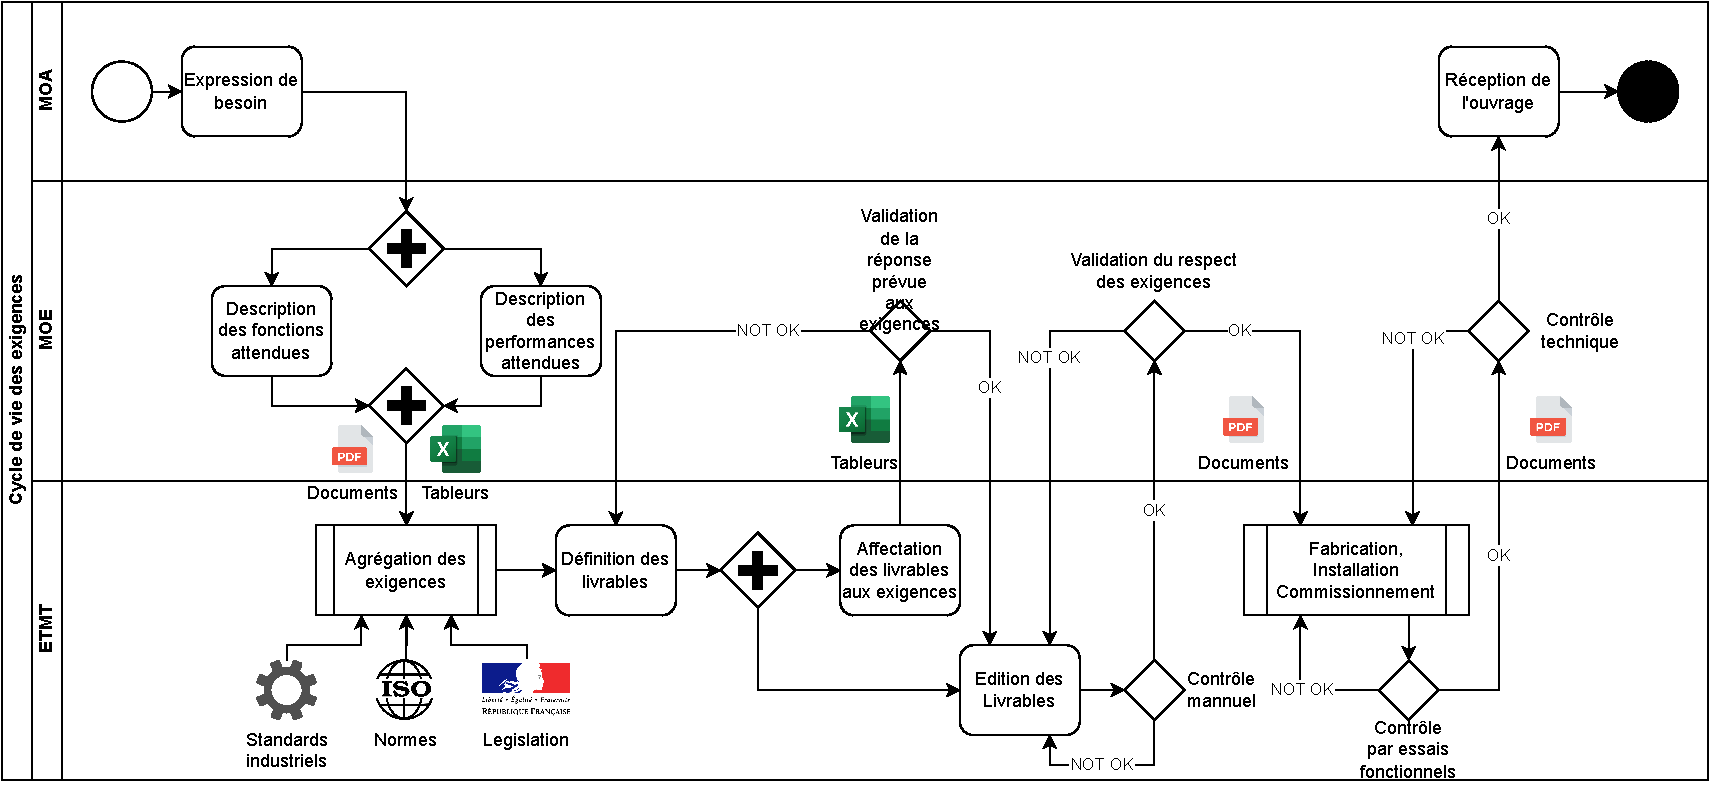
\includegraphics[width=.9\linewidth]{./svg/BPMN-LifeCycle-Exigences-init.pdf}
\caption{\label{fig:org89de545}Macro-processus de traitement des contraintes durant un projet de construction.}
\end{figure}

Comme visible en Figure \ref{fig:org89de545}, la Maitrise d’OuvrAge
 (\protect\hyperlink{gls-9}{\label{gls-9-use-1}MOA}) définit les besoins. Ceux-ci sont précisés par la Maitrise d'Œuvre
 (\protect\hyperlink{gls-10}{\label{gls-10-use-1}MOE}) puis intégrés par l' Entreprise Titulaire d'un Marché de Travaux
 (\protect\hyperlink{gls-11}{\label{gls-11-use-1}ETMT}). Cette dernière est alors responsable de la supervision des contraintes, des moyens d’y répondre, de la réalisation des études et de l'exécution des travaux. Les deux acteurs précédents assurent des rôles d'approbation ou de support. On constate qu’on impose généralement au dernier acteur d’un cycle de conception le respect d’un corpus de contraintes dont il n’a pas participé à l’élaboration. Par ce fonctionnement, l’ensemble des responsabilités semble concentré sur le constructeur.

Les outils informatiques actuels permettent de répondre convenablement aux contraintes techniques. La modélisation procédurale permet de générer des modèles numériques respectant un ensemble de contraintes géospatiales et géométriques \autocite{s.dineshkumarBIMbasedAutomatedSite2015}. La réalisation de notes de calculs, les simulations et les mesures physiques sont des moyens complémentaires permettant de prouver l’atteinte d’un objectif technique \autocite{tomc.borstBIMSimulation2015,galSimulationEnergetiqueDynamique2025a}. Ces aspects sont tout de même chronophages, car ils nécessitent des étapes de configuration et de paramétrage, comparés aux solutions nouvelles employant des modèles génératifs \autocite{chaillouLintelligenceArtificielleAu2021a}. Les configurations sont réalisées généralement par des experts et la vérification des rapports extraits des simulations demande également un haut niveau de technicité \autocite{delsavioVirtualDesignConstruction2022a}. Le plus souvent, les outils sont utilisés en silos et ne permettent pas de partager un environnement de contraintes commun \autocite{moreauConceptionElectriqueQuelles2019a}. Les itérations permettant d’aboutir à une solution viable pour un aspect métier (électrotechnique, mécanique, etc.) peuvent entraîner la mise en défaut de contraintes d’un autre aspect métier \autocite{vandebrugInterdisciplinaryConfigurationMethods2025a}. Il serait intéressant d’établir un cadre d'exécution des vérifications des contraintes partagé pour favoriser l’abandon rapide des itérations aux solutions parasitantes.

Actuellement, il n'existe pas de système permettant d’assurer le respect des contraintes fonctionnelles et organisationnelles à un niveau qualitatif équivalent à ceux destinés aux contraintes techniques. Ce périmètre est alors limité à l'apport en connaissances individuelles et repose entièrement sur un système de confiance pair-à-pair. Ce système de confiance, couplé au cloisonnement des compétences, crée un environnement de doute contraignant les processus d'acceptation en multipliant les contraintes d’approbation. On peut toutefois mentionner l’existence de recherches relatives à la mise en œuvre de protocoles de validation permettant de soulager la charge de la preuve et du manque de confiance entre les parties au moyen de technologies de cryptographie et de chaîne de blocs \autocite{mathewsBIM+BlockchainSolutionTrust2017a}. 
\subsubsection{Focus sur l’électrotechnique et ses contraintes}
\label{sec:org5752bb9}
Les bâtiments contemporains sont parcourus par de nombreux réseaux électriques de différentes natures : signalisation, données, puissance. La diversité de ces réseaux implique une gestion complexe de contraintes diverses et sophistiquées : il peut s'agir d'interface avec le génie climatique sur l'alimentation d'équipements et des remontées de capteurs, de mise en oeuvre de systèmes complexes de détection d'incendies reliés avec les sapeurs pompiers locaux ou encore la réalisation d'un réseau de surveillance et de sécurité assujetti à des dispositions de résilience informatique. La multiplicité des domaines techniques appliqués à la gestion des réseaux électriques augmente la quantité de clauses contractuelles ainsi que le corpus normatif et législatif à prendre en responsabilité par les entreprises. 

Lors de la réalisation des études électrotechniques chez Eiffage Energies Systèmes (EES), les opérations sont découpées au regard des compétences nécessaires à leur aboutissement. Ainsi, un pôle spécialisé en distribution de courant s’occupe de notes de calculs et de schématiques, un autre se spécialise dans les études de conversion de fréquences, une équipe code les programmes d’automatisme, un collaborateur intègre les composants d’automatisme dans les schémas électriques préalablement préparés par le premier pôle présenté, un coordonnateur collecte et met en cohérence les besoins en matières de câbles, un autre pilote l’attribution de code d’identification, un pôle modélise les installations en 3D, certains de ses membres ont une spécialité en mécanique, en électromécanique ou encore en préparation de chantier. 

En zoomant sur cette organisation, nous observons une grande diversité de compétences associées à des référentiels spécifiques. Elles s’étendent par exemple de la mise en oeuvre des normes de sécurité incendie, de l’Eurocode 3 \autocite{icabEurocodesCodesConstructiona} sur la fixation des éléments jusqu’aux habilitations Qualifoudre \autocite{charpentierReferentielPourCertificationa}. Ces éléments sont rarement maîtrisés simultanément. L’empilement des référentiels techniques à respecter entraîne des contraintes en matière de gestion des ressources humaines des projets.

La diversité des équipes permet à l’entreprise de réaliser un large périmètre d’étude sans recourir à des sous-traitants. Cependant, le maintien des compétences en interne associé à leur haute concentration entraîne un risque de perte de compétences en cas d’imprévu. Ce problème implique également des difficultés de vérification interne des études produits lorsqu’une thématique n’est maîtrisée que par une ou deux personnes.

Chaque sous-domaine requiert généralement l’approbation d'un expert intervenant souvent en fin de cycle de conception. Cette intervention peut arriver trop tardivement : une infraction de contrainte critique peut nécessiter le renvoi du projet en amont de la phase de conception et entraîner des surcoûts et des retards. À titre d’exemple, sur un projet d’électrification d’un bassin de maintenance d’un navire, des imprécisions dans les étapes de conception ont conduit à une sous-estimation des besoins en dimensions et en nombre de câbles. Cela a engendré des complexités supplémentaires pour EES lors de la réalisation de son marché de travaux. L’entreprise d’électricité, dès son intégration au projet, a réétudié le dimensionnement des besoins de câbles de façon précise et a fait observer que les caniveaux spécifiés étaient plus de deux fois trop petits pour permettre l’accueil des besoins réels en canalisations électriques. Cette erreur a nécessité le renvoi du projet en bureau d’études pour identifier de nouveaux cheminements et modes de pose.

Un tel enchaînement d'événements pourrait être évité en proposant aux acteurs de la phase de conception des outils interactifs et intuitifs permettant d’éviter en amont les infractions aux contraintes électriques. Il s'agirait de rendre explicites le fonctionnement et les contraintes des différents flux électriques, leurs interférences avec les équipements environnants ainsi que les autres réseaux,leurs contraintes sécuritaires et normatives par des retours visuels et textuels adaptés. Dans ce but, il est important de respecter les critères d'utilisabilité au sens de la norme ISO 9241-11:2018 \autocite{ErgonomieLinteractionHommesysteme2018}, et de vérifier la cohérence avec la démarche cognitive inhérente à la phase de conception, pour chaque acteur concerné. Il serait ainsi possible de garantir le respect de ces contraintes à chaque modification du projet ou à intervalles réguliers à la manière des tests unitaires dont la pratique a été systématisée dans l'industrie du génie logiciel.

La complexification croissante des bâtiments, notamment due à leur informatisation \autocite{DecretNdeg20208872020,SmartReadinessIndicatora}, crée de nouveaux besoins impliquant de nouvelles compétences. Ainsi, sur des projets d’envergure, la multiplicité des besoins en systèmes informatiques est telle qu’il devient nécessaire de composer des équipes d'experts pour en assurer le suivi. Il existe historiquement les systèmes de Gestion Technique du Bâtiment
 (\protect\hyperlink{gls-12}{\label{gls-12-use-1}GTB}), de Gestion Technique Centralisée
 (\protect\hyperlink{gls-13}{\label{gls-13-use-1}GTC}), de sécurité incendie, de Voix, Données et Images
 (\protect\hyperlink{gls-14}{\label{gls-14-use-1}VDI}) et les Système de Contrôle et d'Acquisition de Données
 (\protect\hyperlink{gls-15}{\label{gls-15-use-1}SCADA}). Ceux-ci sont désormais complétés par des systèmes de réseaux IP privés tels que les réseaux Multiprotocol Label Switching
 (\protect\hyperlink{gls-16}{\label{gls-16-use-1}MPLS}), de diffusion de réseaux 5G privés et de divers systèmes d’Internet of Things
 (\protect\hyperlink{gls-17}{\label{gls-17-use-1}IoT}). Ces nouveaux éléments ajoutent des contraintes conséquentes liées aux infrastructures informatiques et à la sécurisation des services.

Lors de la phase d’organisation d’un marché global de performance portant sur la création d’un technicentre, EES a rassemblé une équipe dédiée à la prise en charge du périmètre des technologies de l’information. Elle est missionnée dans la gestion des risques de cybersécurité, l'ingénierie des réseaux informatiques, la conception de centres de données, la mise en œuvre d’environnements de travail virtualisés, dans l’intégration des services applicatifs et pilote les opérations de collecte et d’analyse de données. L’entreprise observe que ces thématiques représentent collectivement un volet important sur le projet mentionné, rivalisant avec les lotissements habituels. 

L'analyse des méthodes actuelles de traitement des contraintes révèle des lacunes significatives, particulièrement en ce qui concerne les contraintes fonctionnelles et organisationnelles. Ces limitations se manifestent avec une acuité particulière dans le domaine de l'électrotechnique, où la complexité croissante des systèmes et la multiplicité des intervenants amplifient les difficultés de coordination et de vérification de conformité. Les défis identifiés illustrent parfaitement les verrous systémiques qui entravent l'efficience des processus de conception et de construction. Face à ces constats, il devient nécessaire de définir des orientations de recherche susceptibles de proposer des solutions pour automatiser et optimiser la gestion des contraintes dans ce secteur spécialisé.
\subsubsection{Retour d'expérience}
\label{sec:org441874b}
\begin{itemize}
\item Trx Master 1 et Master 2
\item Modélisation depuis 2015
\item Intervention sur nombre de projets
\end{itemize}

Parcours perso, ressentis et ambitions.

Sclérosité systémique des lotissements traditionnels
=> Chaines de valeurs traditionnelles devenu rigides et incapable de s'adapter ou d'évoluer à cause de
      la bureaucratisation des procédés ("tamponé, double tamponé\ldots{}" Au service de la France)
      la dérive des régulations (normes, réglements\ldots{})   
      la résistance au changement des collaborateurs
      l'amnésie organisationnelle et l'obsolescence des pratiques
      la déchéance du système de confiance (limites de la preuve par la formation ou par la réputation)
=> Recherche en refonte des organisation ?
=> Identification des leviers

Emergence de nouveaux acteurs 
(informatique et numérique, Les ESN dans la construction ?)
=> Nouveaux outils et moyens de production
=> Besoins, impacts et opportunités

Discorde entre ergonomie et fonctionnalités
Objectif : définir le besoin de simplification, de convergence et d'apport de soin dans l'expérience utilisateur
Ergonomie des interfaces, ergonomie des flux et procédures, charge cognitive \& co
=> Inéficience des ergonomies applicatives et des expériences utilisateurs, dégradées au profit d'une inflation de fonctionnalités
=> Besoin de retrouver de l'abstraction

La réalisation et la maintenance des maquettes numériques, en se contentant de se superposer aux métiers historiques de la construction, court le risque d’évoluer en une forme d’organisation autonome dont l’objectif principal est la pérennisation et le développement de son organisation \autocite{lourauAnalyseInstitutionnelleQuestion1973}. Cette tendance se manifeste d’ores et déjà par la refonte des organisations de projets qui incluent des structures dédiées au \protect\hyperlink{gls-1}{\label{gls-1-use-9}BIM} et composées d’une ligne de management et d’un cadre contractuel adaptés aux seules finalités de cette discipline.

Cette transformation impacte inévitablement des cultures et attitudes historiquement adoptées par les acteurs des entreprises de la construction dont les délais serrés et les objectifs parfois antagonistes favorisent le maintien d’un statu quo au sein des organisations et des pratiques \autocite{lindbladBIMImplementationOrganisational2015,paulagordogregorioContinuiteInformationnelleDans2023}. 

Pourtant, comme l'expriment Hardin \& McCool,
\begin{quote}
Le \protect\hyperlink{gls-1}{\label{gls-1-use-10}BIM} n’est pas un modèle 3D, c’est une méthode de gestion de l’information par le projet. -- Hardin \& McCool, 2019 \autocite{hardinBIMAppliqueAu2019}
\end{quote}


\begin{quote}
The level of information needed defines what is required, when, and why - not how much can be delivered. -- ISO 7817-1, 2023 \autocite{ModelisationInformationsConstruction2024} 
\end{quote}

Après avoir simplifié sa structure, simplifier ses outils et monter en compétences

Ici sourcer : Blender > All car "all-in-one" un peu moins bien c'est mieux que des verticales très maitrisés mais une absence d'interopérabilité => perte de valeur dû à la non continuité des informations, la perte de contexte, etc.
Idem possible : Notion vs MS365, Revit vs AutoCAD et ses "flavours"
etc.

Explorer les bonnes pratiques en IHM, Ui, Ux, définir les "prérequis" 
Explorer le Behavior Driven Design 
\subsubsection{Conclusion}
\label{sec:org8dd1a7a}
Expliquer le besoin de rééquilibrer les responsabilités et d'assainir la base avant de construire, notion de refondation de la chaine de valeur.

Objectif : proposer un cadre de travail scalable à forte valeur ajoutée et identification des rôles et périmètres 
Prérequis avant toute tentative de digitalisation (en 1 : on se remet en question et on balaie devant sa porte)
\begin{itemize}
\item spécialisations horizontales versus verticale
\item parcours de carrières (Expertise, Management, Projet)
\end{itemize}

Explorer la décentralisation de la confiance notamment à travers les ZKP
\subsection{Problématique de recherche}
\label{sec:orgeb53cb4}
Cette thèse s'inscrit dans une démarche de réponse à des enjeux majeurs rencontrés par les entreprises du secteur de la construction \autocite{guillouSegmentationDansEntreprises2003b} et notamment définis par les normes :
\begin{itemize}
\item Management de la qualité (ISO 9001),
\item Gestion des risques (X 50-117),
\item Maîtrise des coûts (X 50-137),
\item Maîtrise des délais (X 50-138),
\item Capitalisation sur l'expérience (X 50-190).
\end{itemize}

Cette thèse va tenter de proposer des pistes permettant de lever les verrous qui freinent l'exécution efficiente de la remontée de conformité en ingénierie de systèmes électriques. Pour ce faire, trois volets seront considérés.

Différentes solutions de l'état de l'art seront étudiées afin de permettre l'extraction dynamique des contraintes fonctionnelles et organisationnelles. Les solutions étudiées seront tirées des domaines de traitement des langues naturelles appliqué aux corpus de textes réglementaires et législatifs ainsi que de l'état de l'art dans le domaine de la création et de l'échange d'ontologies appliquées au \protect\hyperlink{gls-1}{\label{gls-1-use-11}BIM}.

Lorsqu'une contrainte est enfreinte, il est nécessaire de remonter à l'utilisateur non spécialiste la nature de l'infraction, sa ou ses causes et une ou plusieurs suggestions capables de lever l'infraction observée. Les solutions étudiées porteront sur les travaux liés à la conception d'Interfaces Utilisateur (UI) \autocite{Shneiderman2016}, la prise en compte de critères de l'eXpérience Utilisateur (UX) \autocite{Nogier2020} et la réduction de la charge mentale de travail \autocite{longoHumanMentalWorkload2022a,morayMentalWorkloadIts1979a} en situation d'interaction humain-machine. 
Parmi les approches étudiées, celle dite  d'interface écologique fera l'objet d'une attention particulière \autocite{vicenteEcologicalInterfaceDesign1992b,Burns2004}. Le but de telles interfaces est de rendre perceptivement évidentes à l'utilisateur les contraintes et les relations complexes constitutives de l'environnement de travail.

Les outils ne sont pas neutres \autocite{borremansGuideConvivialTools1979a}, ils permettent d'accompagner l'adoption de nouvelles méthodologies de travail. Les méthodes étudiées porteront notamment sur les pratiques agiles adoptées par l'industrie du génie logiciel et sur leur mise en place éventuelle dans le domaine de la construction. Nous étudierons en particulier comment la gestion itérative des modifications successives au projet (versioning) peut influencer l'organisation de la collaboration entre les différents acteurs d'un projet de construction.

Le processus présenté en figure \ref{fig:org89de545} pourra évoluer vers une version allégée dont la figure \ref{fig:org2d77261} propose un exemple.

\begin{figure}[htbp]
\centering
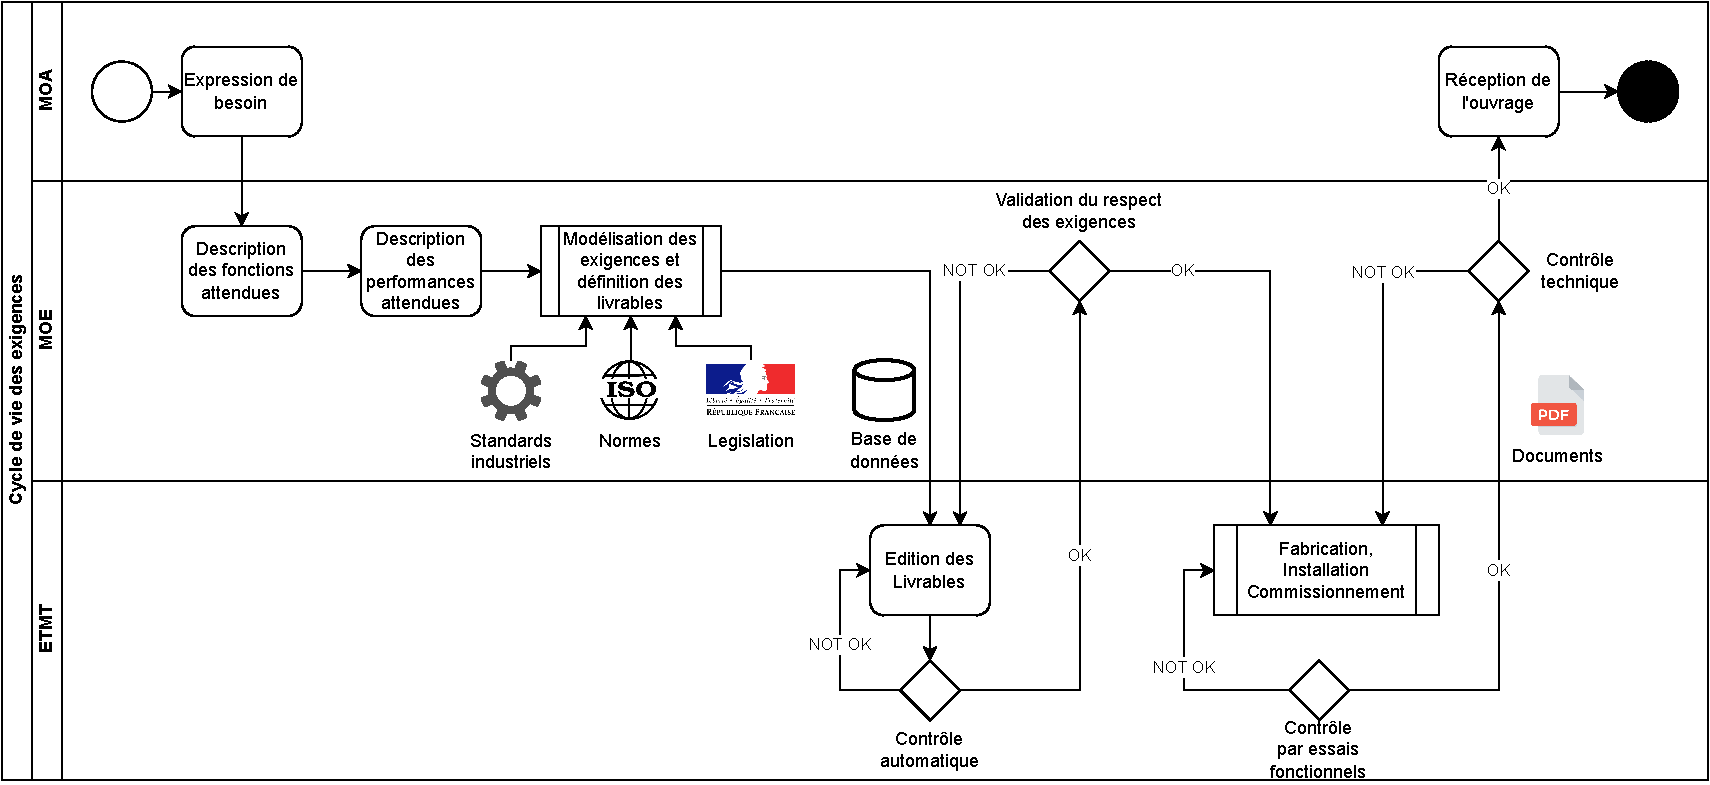
\includegraphics[width=.9\linewidth]{./svg/BPMN-LifeCycle-Exigences-target.pdf}
\caption{\label{fig:org2d77261}Macro-processus de traitement des contraintes durant un projet de construction avec automatisation des vérifications d’études.}
\end{figure}

Question principale :
\begin{itemize}
\item Q0.0 : Comment réduire la charge cognitive liée à la gestion des contraintes en projet de construction ?
\end{itemize}

Questions complémentaires :
\begin{itemize}
\item Q0.1 : Comment créer un environnement de gestion des contraintes hétéroclytes ?
\item Q0.2 : Comment décrire une contrainte en langage naturel ?
\end{itemize}
\subsection{Objectifs et contributions}
\label{sec:org9c2a476}
Présenter la double finalité de la recherche :  
\begin{itemize}
\item scientifique : formaliser un modèle d’interface écologique pour l’aide à la décision sous contraintes ;
\item industrielle : proposer un outil expérimenté dans un contexte réel (EES / poste ferroviaire).
\end{itemize}

Retombées attendues
\begin{itemize}
\item \textbf{Côté laboratoire :} Les résultats attendus sont une méthode générique et une architecture de système sensible aux contraintes, ainsi que des données d'évaluation centrée utilisateur. Des publications scientifiques sont également attendues.
\item \textbf{Côté entreprise :} Les résultats attendus sont l'application de la méthode proposée sur des cas spécifiques à l'entreprise, débouchant sur un prototype de système sensible aux contraintes. Des données d'évaluation technique sont aussi attendues.
\end{itemize}


\begin{table}[htbp]
\caption{Contributions scientifiques}
\centering
\begin{tabular}{ll}
Type & Contribution\\
\hline
Article de conférence & \\
\end{tabular}
\end{table}
\subsection{Organisation du document}
\label{sec:org5302267}
\clearpage
\section{Exploration sectorielle (20p)}
\label{sec:org3139363}
\subsection{Introduction}
\label{sec:org03f10d4}
(Okoli, Tranfield)
\begin{itemize}
\item \textbf{\textbf{Contexte et problématique}} : préciser le champ disciplinaire et la pertinence pratique/organisationnelle.
\item \textbf{\textbf{Objectif scientifique}} : situer la revue comme méthode de recherche en soi, permettant de cartographier un champ et de développer une contribution conceptuelle (typologie, cadre théorique, taxonomie, agenda de recherche).
\item \textbf{\textbf{Pertinence managériale}} : expliquer en quoi la revue éclaire les besoins des organisations et des acteurs.
\end{itemize}
\subsection{Protocole de recherche}
\label{sec:orgb7f2c40}
Research questions
\begin{description}
\item[{\hyperref[orga6d67e2]{RQ1}}] 

\item[{\hyperref[org6b49f3a]{RQ2}}] 
\end{description}

Methode SPIDER
\begin{itemize}
\item \textbf{\textbf{Sample (S)}} : acteurs, organisations, secteurs étudiés (ex. entreprises, managers, équipes projets).
\item \textbf{\textbf{Phenomenon of Interest (PI)}} : pratiques, processus, technologies, comportements managériaux étudiés.
\item \textbf{\textbf{Design (D)}} : types de designs méthodologiques inclus (études de cas, enquêtes, analyses qualitatives, etc.).
\item \textbf{\textbf{Evaluation (E)}} : indicateurs ou dimensions étudiées (performance, adoption, impacts organisationnels).
\item \textbf{\textbf{Research type (R)}} : types de recherche acceptés (empirique, théorique, revue existante).
\end{itemize}

Research string
\begin{itemize}
\item Construction des équations avec opérateurs booléens et synonymes.
\end{itemize}

\begin{listing}[htbp]
\begin{Code}
\begin{Verbatim}
\color{EFD}("knowledge management" \EFk{OR} "organizational learning") \EFk{AND} ("digital transformation" \EFk{OR} "IT adoption")
\end{Verbatim}
\end{Code}
\caption{\label{lst:org1d894c5}Requête générique}
\end{listing}

\begin{table}[htbp]
\caption{\label{tab:orga79d12b}Déclinaison de la requête générique par bases de données ciblées}
\centering
\begin{tabular}{ll}
Name & Query\\
\hline
Scopus & \\
Web of Science & \\
Business Source Complete (EBSCO) & \\
ScienceDirect & \\
Google Scholar & \\
\end{tabular}
\end{table}

Littérature grise
\begin{itemize}
\item Rapports professionnels, thèses, working papers.
\item Justification de l’inclusion ou exclusion.
\end{itemize}

Processus de sélection (Tranfield)
\begin{enumerate}
\item \textbf{\textbf{Recherche initiale}} → collecte des références.
\item \textbf{\textbf{Déduplication}}.
\item \textbf{\textbf{Screening par titre et résumé}}.
\item \textbf{\textbf{Screening par texte intégral}}.
\item \textbf{\textbf{Validation inter-évaluateurs}} (au moins deux chercheurs, résolution des désaccords par consensus).
\end{enumerate}

Critères d’inclusion et d'exclusion
\begin{itemize}
\item Inclusion : articles académiques en gestion/SHS, période temporelle définie, pertinence thématique.
\item Exclusion : non revu par les pairs (sauf gris justifié), hors champ, doublons.
\end{itemize}

Formulaire d’extraction (Okoli)
\begin{itemize}
\item Identifiant (ID)
\item Référence bibliographique
\item Contexte (secteur, pays, type d’organisation)
\item Méthodologie de l’étude
\item Résultats principaux
\item Concepts/variables mobilisés
\item Contribution théorique ou pratique
\end{itemize}

Évaluation de la qualité (Okoli)
\begin{itemize}
\item Pertinence théorique (forte/moyenne/faible).
\item Validité méthodologique (forte/moyenne/faible).
\item Clarté de la contribution.
\end{itemize}
\subsection{Résultats de recherche}
\label{sec:org882d1a1}
Nombre d’articles identifiés, filtrés, exclus, inclus.

\textbf{PRISMA 2020 flow diagram} for new systematic reviews which included searches of databases and registers only
\begin{itemize}
\item Présenter le flux : articles identifiés, retenus, exclus, inclus.
\item Fournir la checklist 2020 PRISMA-RR (traçabilité).
\item Appliquer les interim guidance pour les Rapid Reviews issues du groupe Cochrane : expliciter les écarts méthodologiques, les raccourcis, la justification de ces choix.
\item Inclure un diagramme de flux (identification → sélection → inclusions) adapté au contexte RR.
\item Intégrer les éléments de publication / éthique : auteurs, contributions, relecteurs, conflits d’intérêt.
\item Mention explicite du fait que PRISMA-RR est en développement et que ce rapport est conforme aux principes provisoires.
\end{itemize}
\url{https://pmc.ncbi.nlm.nih.gov/articles/PMC12013547}
\url{https://pubmed.ncbi.nlm.nih.gov/39038926}
\url{https://www.equator-network.org/wp-content/uploads/2018/02/PRISMA-RR-protocol.pdf}
\subsection{Analyses des résultats}
\label{sec:org23b554e}
\begin{itemize}
\item \textbf{\textbf{Analyse descriptive}} : nombre d’articles, évolution temporelle, répartition par journaux/méthodes.
\item \textbf{\textbf{Analyse thématique}} : regroupement des contributions en catégories conceptuelles.
\item \textbf{\textbf{Construction conceptuelle}} : cadre, typologie, ou modèle explicatif.
\item \textbf{\textbf{Agenda de recherche}} : identification des lacunes et pistes futures.
\end{itemize}
\subsection{Discussion}
\label{sec:org31624a3}
\begin{itemize}
\item \textbf{\textbf{Synthèse des apports}} : résumé des résultats majeurs.
\item \textbf{\textbf{Implications théoriques}} : enrichissement du corpus scientifique en gestion.
\item \textbf{\textbf{Implications pratiques}} : recommandations pour les acteurs managériaux.
\item \textbf{\textbf{Limites méthodologiques}} : biais de sélection, couverture des bases, etc. Risques de biais de publication, Risques liés à l’échantillonnage ou aux bases de données, Stratégies d’atténuation (diversification, double codage).
\item \textbf{\textbf{Perspectives}} : agenda pour futures recherches.
\end{itemize}
\subsection{Conclusion}
\label{sec:org4d7eed3}
\clearpage
\section{Etat de l'art (80p)}
\label{sec:org5999d23}
\subsection{Introduction}
\label{sec:orgc8ad11a}

\subsubsection{Background}
\label{sec:org2f5715c}
\subsubsection{Business rules}
\label{sec:org427a71d}

\subsubsection{Ecological interface design}
\label{sec:org4e43ea5}
\subsection{Protocol de recherche}
\label{sec:org3ea09d4}
\subsubsection{Questions de recherche}
\label{sec:orgac27853}
Questions principales
\begin{description}
\item[{\label{orga6d67e2}RQ1}] Comment les principes de l’Ecological Interface Design ont-ils été appliqués à la représentation visuelle de règles métiers ou de systèmes de contraintes ?
\item[{\label{org6b49f3a}RQ2}] Quelles approches conceptuelles, méthodologiques ou techniques ont été mobilisées pour rendre visibles ou compréhensibles les états d’une règle métier (valide, bloquée, inactive, en alerte, etc.) ?
\item[{\label{org133b723}RQ3}] Quels modèles cognitifs, ergonomiques ou informationnels ont été mobilisés pour adapter la visualisation des règles métiers au contexte d’usage (rôle utilisateur, environnement, phase de travail, niveau d’expertise, etc.) ?
\end{description}

Questions secondaires
\begin{description}
\item[{\label{org44f66f4}RQ4}] Quels types de métaphores visuelles ou structures d’information ont été proposés pour représenter la complexité des interdépendances entre règles métiers (hiérarchie, causalité, propagation d’état) ?
\item[{\label{orga733c3a}RQ5}] Quels domaines applicatifs ont le plus exploré ces approches (ex. : systèmes industriels, ingénierie, santé, finance, administration, etc.) et dans quelles finalités (supervision, décision, audit, apprentissage) ?
\item[{\label{org244ddbb}RQ6}] Quelles sont les limites identifiées dans la littérature concernant l’applicabilité des principes EID à des systèmes de règles dynamiques (ex. : règles générées, apprises, modifiées en temps réel) ?
\item[{\label{org9ab74c7}RQ7}] Quels modèles d’évaluation (performance, charge cognitive, compréhension, décision) ont été employés pour mesurer l’efficacité de ces interfaces écologiques appliquées aux règles métiers ?
\end{description}


\begin{TABLE}
\begin{center}
\begin{tabular}{lll}
\hline
Element & Definition & Keywords\\
\hline
\textbf{\textbf{Population}} &  & \\
\textbf{\textbf{Intervention}} &  & \texttt{ecological interface design}, \texttt{EID}\\
\textbf{\textbf{Comparison}} & Non utilisé & \\
\textbf{\textbf{Outcome}} &  & \\
\textbf{\textbf{Context}} &  & \\
\hline
\end{tabular}
\end{center}
\caption{\label{org198828c}Methode PICOC}
\end{TABLE}
\paragraph*{Quality assessment criteria}
\label{sec:org71f55c2}
Justification des choix de mots-clés.

L'identification des mots clés permet de préparer la requête des bases de données. Le processus de collecte est illustré par la figure \ref{fig:org7aa5d9a}.

\begin{figure}[htbp]
\centering
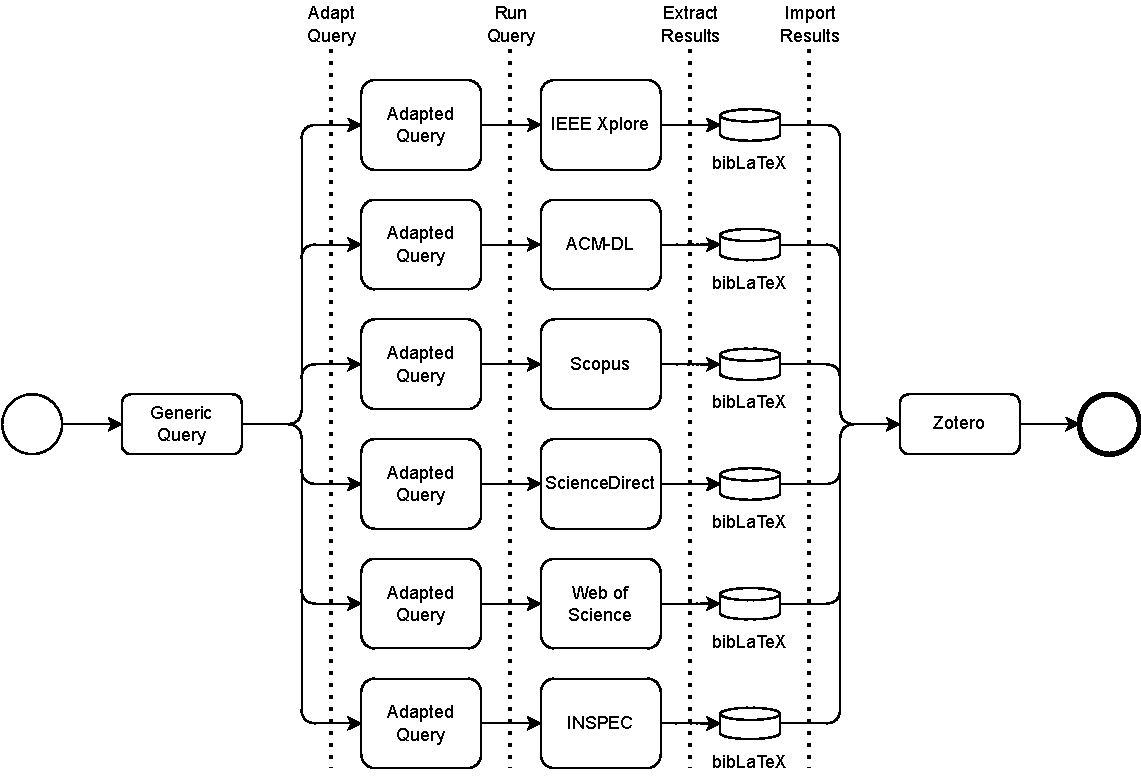
\includegraphics[width=.9\linewidth]{./svg/slr-data-collect.pdf}
\caption{\label{fig:org7aa5d9a}Processus de collecte des données}
\end{figure}

La requête booléenne générique intégrant les mots-clés issus du tableau \ref{org198828c} est présentée par le bloc de code \ref{lst:org693ef2e}. Sa structure suit l’ordre logique : \textbf{Population \(\land\) Intervention \(\land\) Outcome \(\land\) Context}.

\begin{listing}[htbp]
\begin{Code}
\begin{Verbatim}
\color{EFD}\EFcd{--} \EFc{POPULATION: Interfaces, cognition, visualization}
("human-machine interface" \EFk{OR} "human computer interaction" \EFk{OR} "human centered interaction" \EFk{OR} "HMI" \EFk{OR} "HCI")
\EFcd{--} \EFc{INTERVENTION: Ecological Interface Design}
\EFk{AND} ("ecological interface design" \EFk{OR} "EID")
\EFcd{--} \EFc{OUTCOME: cognitive and decision-related outcomes}
\EFk{AND} ("situational awareness" \EFk{OR} "context sensitivity" \EFk{OR} "cognitive load" \EFk{OR} "usability" \EFk{OR} "mental workload" \EFk{OR} "\EFb{user} performance" \EFk{OR} "task performance" \EFk{OR} "error reduction" \EFk{OR} "cognitive efficiency")
\EFcd{--} \EFc{CONTEXT: construction and engineering disciplines}
\EFk{AND} ("construction industry" \EFk{OR} "civil" \EFk{OR} "structural" \EFk{OR} "geotechnical" \EFk{OR} "hydraulic" \EFk{OR} "transport" \EFk{OR} "mechanical" \EFk{OR} "plumbing" \EFk{OR} "sanitary" \EFk{OR} "HVAC"  \EFk{OR} "heating" \EFk{OR} "ventilation" \EFk{OR} "air conditioning" \EFk{OR} "cooling" \EFk{OR} "climate" \EFk{OR} "environmental" \EFk{OR} "electrical" \EFk{OR} "power" \EFk{OR} "energy" \EFk{OR} "lighting" \EFk{OR} "acoustical" \EFk{OR} "thermal" \EFk{OR} "fire safety" \EFk{OR} "industrial" \EFk{OR} "maintenance" \EFk{OR} "construction management" \EFk{OR} "urban" \EFk{OR} "infrastructure")
\end{Verbatim}
\end{Code}
\caption{\label{lst:org693ef2e}Requête générique}
\end{listing}

Les bases de données intérogées sont :
\begin{enumerate}
\item IEEE Xplore
\item ACM Digital Library : The ACM Guide to Computing Literature collection
\item Scopus
\item ScienceDirect
\item Web of Science
\item INSPEC (via Engineering Village or ProQuest)
\end{enumerate}

La requête générique est ainsi adaptée à chaque base de données et les variantes sont présentées par le tableau \ref{org34e83da}

\begin{TABLE}
\begin{center}
\begin{tabular}{ll}
\hline
Base de données & Requête\\
\hline
IEEE Xplore & \Small{"All Metadata":(("human-machine interface" OR "human computer interaction" OR "HMI" OR "HCI") AND ("ecological interface design" OR "EID" OR "ecological design") AND ("situational awareness" OR "context sensitivity" OR "cognitive load" OR "usability" OR "mental workload" OR "user performance" OR "task performance" OR "error reduction" OR "cognitive efficiency") AND (("construction industry" OR "civil engineering" OR "structural engineering" OR "geotechnical engineering" OR "hydraulic engineering" OR "transport engineering" OR "mechanical engineering" OR "plumbing" OR "sanitary engineering" OR "HVAC" OR "heating ventilation air conditioning" OR "climate engineering" OR "environmental engineering" OR "electrical engineering" OR "power engineering" OR "energy engineering" OR "lighting engineering" OR "building physics" OR "acoustical engineering" OR "thermal engineering" OR "fire safety engineering" OR "industrial engineering" OR "maintenance engineering" OR "construction management" OR "architecture" OR "urban engineering" OR "public works" OR "infrastructure engineering")))}\\
\hline
ACM-DL & \Small{("human-machine interface" OR "human computer interaction" OR "HMI" OR "HCI") AND ("ecological interface design" OR "EID" OR "ecological design") AND ("situational awareness" OR "context sensitivity" OR "cognitive load" OR "usability" OR "mental workload" OR "user performance" OR "task performance" OR "error reduction" OR "cognitive efficiency") AND ("construction industry" OR "civil engineering" OR "structural engineering" OR "geotechnical engineering" OR "hydraulic engineering" OR "transport engineering" OR "mechanical engineering" OR "plumbing" OR "sanitary engineering" OR "HVAC" OR "heating ventilation air conditioning" OR "climate engineering" OR "environmental engineering" OR "electrical engineering" OR "power engineering" OR "energy engineering" OR "lighting engineering" OR "building physics" OR "acoustical engineering" OR "thermal engineering" OR "fire safety engineering" OR "industrial engineering" OR "maintenance engineering" OR "construction management" OR "architecture" OR "urban engineering" OR "public works" OR "infrastructure engineering")}\\
\hline
Scopus & \Small{TITLE-ABS-KEY(("human-machine interface" OR "human computer interaction" OR "HMI" OR "HCI") AND ("ecological interface design" OR "EID" OR "ecological design") AND ("situational awareness" OR "context sensitivity" OR "cognitive load" OR "usability" OR "mental workload" OR "user performance" OR "task performance" OR "error reduction" OR "cognitive efficiency") AND (("construction industry" OR "civil engineering" OR "structural engineering" OR "geotechnical engineering" OR "hydraulic engineering" OR "transport engineering" OR "mechanical engineering" OR "plumbing" OR "sanitary engineering" OR "HVAC" OR "heating ventilation air conditioning" OR "climate engineering" OR "environmental engineering" OR "electrical engineering" OR "power engineering" OR "energy engineering" OR "lighting engineering" OR "building physics" OR "acoustical engineering" OR "thermal engineering" OR "fire safety engineering" OR "industrial engineering" OR "maintenance engineering" OR "construction management" OR "architecture" OR "urban engineering" OR "public works" OR "infrastructure engineering")))}\\
\hline
ScienceDirect & \Small{TITLE-ABS-KEY(("human-machine interface" OR "human computer interaction" OR "HMI" OR "HCI") AND ("ecological interface design" OR "EID" OR "ecological design") AND ("situational awareness" OR "context sensitivity" OR "cognitive load" OR "usability" OR "mental workload" OR "user performance" OR "task performance" OR "error reduction" OR "cognitive efficiency") AND (("construction industry" OR "civil engineering" OR "structural engineering" OR "geotechnical engineering" OR "hydraulic engineering" OR "transport engineering" OR "mechanical engineering" OR "plumbing" OR "sanitary engineering" OR "HVAC" OR "heating ventilation air conditioning" OR "climate engineering" OR "environmental engineering" OR "electrical engineering" OR "power engineering" OR "energy engineering" OR "lighting engineering" OR "building physics" OR "acoustical engineering" OR "thermal engineering" OR "fire safety engineering" OR "industrial engineering" OR "maintenance engineering" OR "construction management" OR "architecture" OR "urban engineering" OR "public works" OR "infrastructure engineering")))}\\
\hline
Web of Science & \Small{TS=(("human-machine interface" OR "human computer interaction" OR "HMI" OR "HCI") AND ("ecological interface design" OR "EID" OR "ecological design") AND ("situational awareness" OR "context sensitivity" OR "cognitive load" OR "usability" OR "mental workload" OR "user performance" OR "task performance" OR "error reduction" OR "cognitive efficiency") AND (("construction industry" OR "civil engineering" OR "structural engineering" OR "geotechnical engineering" OR "hydraulic engineering" OR "transport engineering" OR "mechanical engineering" OR "plumbing" OR "sanitary engineering" OR "HVAC" OR "heating ventilation air conditioning" OR "climate engineering" OR "environmental engineering" OR "electrical engineering" OR "power engineering" OR "energy engineering" OR "lighting engineering" OR "building physics" OR "acoustical engineering" OR "thermal engineering" OR "fire safety engineering" OR "industrial engineering" OR "maintenance engineering" OR "construction management" OR "architecture" OR "urban engineering" OR "public works" OR "infrastructure engineering")))}\\
\hline
INSPEC & \Small{(TI=("human-machine interface" OR "human computer interaction" OR "HMI" OR "HCI")) AND (TI=("ecological interface design" OR "EID" OR "ecological design")) AND (TI=("situational awareness" OR "context sensitivity" OR "cognitive load" OR "usability" OR "mental workload" OR "user performance" OR "task performance" OR "error reduction" OR "cognitive efficiency") OR AB=("situational awareness" OR "context sensitivity" OR "cognitive load" OR "usability" OR "mental workload" OR "user performance" OR "task performance" OR "error reduction" OR "cognitive efficiency")) AND (TI=("construction industry" OR "civil engineering" OR "structural engineering" OR "geotechnical engineering" OR "hydraulic engineering" OR "transport engineering" OR "mechanical engineering" OR "plumbing" OR "sanitary engineering" OR "HVAC" OR "heating ventilation air conditioning" OR "climate engineering" OR "environmental engineering" OR "electrical engineering" OR "power engineering" OR "energy engineering" OR "lighting engineering" OR "building physics" OR "acoustical engineering" OR "thermal engineering" OR "fire safety engineering" OR "industrial engineering" OR "maintenance engineering" OR "construction management" OR "architecture" OR "urban engineering" OR "public works" OR "infrastructure engineering") OR AB=("construction industry" OR "civil engineering" OR "structural engineering" OR "geotechnical engineering" OR "hydraulic engineering" OR "transport engineering" OR "mechanical engineering" OR "plumbing" OR "sanitary engineering" OR "HVAC" OR "heating ventilation air conditioning" OR "climate engineering" OR "environmental engineering" OR "electrical engineering" OR "power engineering" OR "energy engineering" OR "lighting engineering" OR "building physics" OR "acoustical engineering" OR "thermal engineering" OR "fire safety engineering" OR "industrial engineering" OR "maintenance engineering" OR "construction management" OR "architecture" OR "urban engineering" OR "public works" OR "infrastructure engineering"))}\\
\hline
\end{tabular}
\end{center}
\caption{\label{org34e83da}Déclinaison de la requête générique par bases de données ciblées}
\end{TABLE}

Nous limitons la collecte d'articles à une profondeur de 10 ans soit entre le 2015-01-01 et le 2025-01-01. Seuls les articles de revues et de colloque en anglais, associés à l'interraction humain-machine sont retenus.
Nous écartons les articles non revues par les pairs, les articles incomplets et ceux sans résultats empiriques.
L'opération de déduplication est réalisée sur Zotero.
\subsubsection{Processus de recherche}
\label{sec:orgfaa9b5b}
Recherche initiale → collecte des résultats → exportation (BibTeX, CSV).
Déduplication (Zotero, EndNote, Mendeley, etc.).

Les articles sont préparés puis sélectionnés en suivant le processus présenté en figure [[ .
Automatique (Action tag, plugin, etc.)
\begin{description}
\item[{Etape 1}] Déduplication \texttt{(merge-entries (:where (= :DOI :Title)))}
\item[{Etape 2}] Filtration \texttt{(delete-entries (:where (and (< :date "2015-01-01") (not (= :langue "en")))))}
\end{description}

Mannuel systématique
\begin{description}
\item[{Etape 3}] non revues par les pairs, incomplets, sans résultats empiriques.
\end{description}

Mannuel collégial
\begin{description}
\item[{Étape 4}] filtrage par titre et résumé.
\item[{Étape 5}] filtrage par texte intégral.
\item[{Étape 3}] validation inter-évaluateurs (au moins deux chercheurs).
\end{description}
\subsubsection{Formulaire d’extraction}
\label{sec:org66373b4}
Champs obligatoires :
    Identifiant (ID)
    Référence bibliographique complète
    Année de publication
    Contexte (population, domaine, technologie)
    Méthodologie de l’étude
    Résultats principaux (Outcome)
    Limites rapportées
\subsubsection{Évaluation de la qualité}
\label{sec:orgb1087d1}
Checklist PRISMA, indiquer la localisation de chaque item dans le rapport final.

Checklist qualité (exemple) :
    Clarté des objectifs : oui/non
    Méthodologie décrite : oui/non
    Données empiriques disponibles : oui/non
    Validité des résultats : élevé/moyen/faible
\subsubsection{Schéma de sélection}
\label{sec:org6184448}
Nombre d’articles identifiés, filtrés, exclus, inclus.

\textbf{PRISMA 2020 flow diagram} for new systematic reviews which included searches of databases and registers only
\subsection{Analysis and results}
\label{sec:org95e9874}
Méthodes d’analyse
    Quantitative (comptages, distributions, tendances temporelles).
    Qualitative (analyse thématique, catégorisation, taxonomie).
    Meta-analysis (si applicable).
\subsection{Wrapping up}
\label{sec:org225a841}
\subsubsection{General discussion}
\label{sec:org4731491}
Contribution scientifique :
    Lacunes identifiées
    Etat de l’art consolidé.
Contribution pratique :
    Recommandations
    Implications pour les chercheurs et praticiens.
Limites méthodologiques du protocole.
\subsubsection{Recommendations}
\label{sec:org3878fef}
\subsection{Treats to validity}
\label{sec:org9c995d7}
Risques de biais de publication.
Risques liés à l’échantillonnage ou aux bases de données.
Stratégies d’atténuation (diversification, double codage).
\subsection{Research opportunity}
\label{sec:orgd83c84b}

\subsection{Conclusion}
\label{sec:orgabd6f01}
\clearpage
\section{Problématique de recherche (20p)}
\label{sec:orgb82d1b1}
\subsection{Introduction}
\label{sec:org1cd74bc}
Rappel : après l’état de l’art, une zone non résolue est identifiée (ex. gestion des contraintes via IHM écologiques).
Objectif : transformer cette zone non résolue en une problématique scientifique explicite.
Cadres mobilisés : Whetten, Alvesson \& Sandberg, QQOQCCP, RCA.
\subsection{Définition de la problématique}
\label{sec:org7aa0782}
(Whetten, 1989)
What : quels éléments précis posent problème (ex. multiplicité et incohérence des contraintes projet).
How : comment ces éléments interagissent ou produisent des effets négatifs.
Why : pourquoi il est crucial d’y répondre (enjeux théoriques + pratiques).
Who / Where / When : quels acteurs, contextes, phases du projet sont concernés.
\subsection{Analyse critique}
\label{sec:org634fe81}
(Problematization – Alvesson \& Sandberg, 2011)
Identifier les hypothèses dominantes dans la littérature (ex. “les contraintes sont gérables par les méthodes classiques de planification”).
Montrer leurs limites ou leur obsolescence.
Créer une tension : pourquoi ces hypothèses ne suffisent plus dans les environnements actuels.
Reformuler la problématique comme une contradiction non résolue.
\subsection{Déclinaison opérationnelle}
\label{sec:org6b8ea67}
(QQOQCCP / 5W1H)
Quoi : description détaillée du problème organisationnel.
Qui : acteurs directement et indirectement affectés.
Où : environnement spécifique (projets complexes, systèmes socio-techniques).
Quand : temporalité critique (conception, exécution, suivi).
Comment : limites des solutions actuelles.
Combien : ampleur mesurée (coûts, délais, incidents).
Pourquoi : justification du caractère central du problème.
\subsection{Analyse des causes profondes}
\label{sec:org76b55dc}
(RCA / Ishikawa / 5 Why’s)
Identification des sources techniques, organisationnelles, cognitives.
Mise en évidence de l’origine structurelle du problème : absence de cadre unifié pour gérer, résoudre et préserver les contraintes.
\subsection{Proposition de recherche}
\label{sec:org0ba41ff}
Formulation claire, nette et précise de la problématique en une phrase :
« Comment concevoir une pratique organisationnelle et un cadre outillé permettant de modéliser, résoudre et préserver les contraintes dans les projets complexes, en intégrant des interfaces écologiques adaptées aux acteurs ? »

Positionner cette formulation comme le pivot entre état de l’art et théorisation.
\subsubsection{Questions de recherche}
\label{sec:orgbbd7ba8}
Question principale : Comment développer une approche d'ingénierie par les contraintes pour améliorer la conception et la validation des systèmes de génie électrique ?

Questions secondaires :
\begin{itemize}
\item Quels mécanismes de vérification formelle intégrer dans cette approche ?
\item Comment remonter aux utilisateurs [\ldots{}] (IHM)
\item Comment assurer la traçabilité des contraintes techniques ?
\item Quelle est l'efficacité de cette approche comparée aux méthodes traditionnelles ?
\end{itemize}
\subsubsection{Approche méthodologique}
\label{sec:orga0a6261}
\subsection{Discussion}
\label{sec:org8b7848f}
Montrer que la problématique n’est pas une simple lacune, mais une tension théorique + enjeu pratique majeur.
Mettre en évidence la valeur de cette problématique pour :
les chercheurs (nouvelle théorie),
les praticiens (nouveaux outils).
\subsection{Conclusion}
\label{sec:org0491dde}
Récapitulatif de la problématique formalisée.
Insistance sur son rôle structurant pour la suite (théorisation → implémentation → évaluation).
\clearpage
\section{Fondements théoriques (20p)}
\label{sec:orgbfe74a4}
\subsection{Méthodologie}
\label{sec:org4f2b8e7}
\subsubsection{Stratégie de recherche}
\label{sec:org7ca159b}
La stratégie repose sur la Design Science Research (DSR) (Hevner et al., 2004 ; Peffers et al., 2007 ; Gregor \& Jones, 2007) comme ancrage principal pour construire une théorie de conception en gestion de projet.
Elle est enrichie par :
\begin{itemize}
\item l’Action Design Research (ADR) (Sein et al., 2011) afin d’intégrer les utilisateurs dans la boucle de recherche,
\item le cadre CIMO / Realist Evaluation (Pawson \& Tilley, 1997 ; Denyer et al., 2008) pour structurer les mécanismes explicatifs,
\item l’approche processuelle de Langley (1999) pour représenter la dynamique organisationnelle et ses évolutions.
\end{itemize}
\subsubsection{Socles théoriques}
\label{sec:orgffbf50e}
Théories des artefacts de conception et de l’action (DSR, ADR).
Théories causales mécanistes (CIMO).
Théorisation processuelle (Langley).
Bases en sciences de gestion : routines organisationnelles (Pentland \& Feldman), Knowledge Management (Nonaka, Davenport), interfaces écologiques (Vicente), théorie des jeux, graphes.
\paragraph*{{\bfseries\sffamily TODO} Théories de l’interface écologique}
\label{sec:orgd2f42d1}
Décrire les principes de l’Ecological Interface Design (Vicente, 1999).  
Expliquer les notions de visibilité, affordance, abstraction hierarchy et situation awareness.
\paragraph*{{\bfseries\sffamily TODO} Sensibilité au contexte et cognition située}
\label{sec:orgd56197d}
Définir les dimensions de contexte (utilisateur, tâche, environnement, système).  
Citer Dey \& Abowd (2000), Kaptelinin \& Nardi (2006), Hollnagel (2002).
\paragraph*{{\bfseries\sffamily TODO} Visualisation et interaction pour la négociation de contraintes}
\label{sec:orge5e48a3}
Présenter les approches de visualisation : overview + zoom + filter + details (Shneiderman, 1996).  
Décrire les besoins de représentation et d’interaction pour la compréhension et la négociation.
\subsubsection{Organisation}
\label{sec:org9f6b774}
La méthodologie est organisée en quatre parties :
\begin{itemize}
\item Définition des objectifs (DSR + ADR)
\item Principes de conception (DSR)
\item Mécanismes causaux (CIMO)
\item Dynamiques processuelles (Langley)
\end{itemize}
\subsection{Définition des objectifs}
\label{sec:orgfa7e6c6}
\begin{itemize}
\item Structurer les objectifs de recherche en six étapes (problem identification, objectifs, design, démonstration, évaluation, communication) \autocite[et al. (2007)]{Peffers}.
\item Garantir la pertinence (problèmes issus du terrain) et la rigueur scientifique (bases théoriques) \autocite[et al. (2004)]{Hevner}.
\item Formuler les objectifs conjointement avec les praticiens, en laboratoire puis en contexte industriel \autocite[et al. (2011) (ADR)]{Sein}.
\end{itemize}
\subsection{Principes de conception}
\label{sec:org9d70ee8}
Structuration des principes \autocite[\& Jones (2007)]{Gregor} :
\begin{itemize}
\item But \& portée : Développer une pratique organisationnelle de gestion de projet qui permet de modéliser, résoudre et préserver les contraintes, tout en assurant traçabilité, faisabilité et adaptation continue.
\item Constructs : Acteur, rôle, objet-projet, contrainte, test, graphe de dépendances, mécanisme de propagation, événement, log, interface écologique.
\item Principes de forme et de fonction (unicité, traçabilité, feedback en temps réel)
\begin{itemize}
\item Unicité : une contrainte exprimée en langage contrôlé correspond à une méthode exécutable unique.
\item Traçabilité totale : lien continu du texte utilisateur jusqu’aux logs d’exécution.
\item Écologie de l’interface : feedback visuel et immédiat des contraintes et écarts.
\end{itemize}
\item Principes d’implémentation (pipeline CNL → Graphe → Solveur → IHM)
\item Traduction des objectifs en principes testables et en artefacts concrets (modèles, prototypes).
\item Intégration de la co-construction (ADR) pour que ces principes soient ajustés en continu avec les utilisateurs.
\end{itemize}

Justificatory knowledge : S’appuie sur la littérature en routines organisationnelles, gestion des connaissances (SECI), écologie des interfaces (EID), planification par contraintes (TOC/PERT/CPM), théorie des jeux et graphes.
\subsection{Mécanismes causaux}
\label{sec:orga7659c7}
Utilisation du cadre CIMO (Denyer et al., 2008 ; Pawson \& Tilley, 1997) pour exprimer les mécanismes :
\begin{itemize}
\item Contexte (type de projet, maturité organisationnelle)
\item Intervention (instanciation du graphe de contraintes, IHM écologique)
\item Mécanisme (propagation, négociation, préservation via logs/tests)
\item Outcome (réduction du temps de résolution, meilleure conformité, traçabilité accrue)
\end{itemize}

Exemple
\begin{verbatim}
Dans un projet à forte complexité contractuelle (C), l’instanciation d’un pipeline CNL→Graphe (I) active le mécanisme de détection précoce des conflits (M), réduisant le temps moyen de résolution (O).
\end{verbatim}
\subsection{Dynamiques processuelles}
\label{sec:org6018c8b}
Théoriser les dynamiques organisationnelles \autocite[(1999)]{Langley}.
Méthodes utilisées :
\begin{itemize}
\item Temporal bracketing (séquençage des phases contraintes/tests).
\item Visual mapping (diagrammes Unified Model Language
 (\protect\hyperlink{gls-18}{\label{gls-18-use-1}UML}), System Model Language
 (\protect\hyperlink{gls-19}{\label{gls-19-use-1}SysML}), Business Process Model and Notation
 (\protect\hyperlink{gls-20}{\label{gls-20-use-1}BPMN}) pour modéliser les processus).
\item Narrative strategies (construction d’histoires organisationnelles reliant données empiriques et mécanismes théorisés).
\end{itemize}

Apport : démonstration que la pratique organisationnelle évolue par itérations, au-delà d’une simple modélisation statique.
\subsection{Formulation finalisée de la théorie}
\label{sec:orgc08a18c}
(Design Theory Statement)

Conformément à Gregor \& Jones (2007), la formulation finale de la théorie issue de l’étude peut être structurée en huit éléments. Ci-dessous un exemple de rédaction, que vous raffinerez ensuite à partir des résultats empiriques :

Proposition simple :
\begin{verbatim}
When working on a complex project, any actor will benefit from an ecological HCI design to manage their business rules.
\end{verbatim}

Théorie :
\begin{verbatim}
In complex projects (Where), actors with decision or coordination roles (Who), when provided with an ecological HCI (How) integrating executable business rules (What), during planning and monitoring phases (When), will experience a measurable reduction in resolution time (How much) and increased compliance (Outcome), because mechanisms of visibility, propagation, and traceability (Why) support better coordination across actors (CIMO).
\end{verbatim}
\subsection{Discussion}
\label{sec:orgff9075c}

\subsection{Conclusion}
\label{sec:orga630bca}
Le chapitre aboutit à une architecture de théorisation hybride et multi-niveaux :
Macro-niveau (DSR/ADR) : définition et validation itérative d’une design theory.
Mésos-niveau (CIMO) : formalisation des mécanismes causaux.
Micro-niveau (Langley) : représentation des processus et routines dans le temps.
\clearpage
\section{Taxonomie des contraintes (20p)}
\label{sec:orgcae9582}
\subsection{Définition de contrainte}
\label{sec:org6693969}
À l’origine, contraindre et contrainte évoquent l’idée d’une pression exercée pour restreindre la liberté d’action d’une personne \autocite{CONTRAINTEEtymologieCONTRAINTE}. Dans le langage courant, une contrainte désigne tout ce qui force ou limite la liberté d’action \autocite{DefinitionContrainte}. Par extension, le mot s’applique à toute obligation ou règle à laquelle on doit se plier et qui réduit le champ de liberté.

En outre, certains domaines techniques ont des acceptions spécifiques du terme. En droit, une contrainte peut désigner un acte coercitif \autocite{DefinitionContrainte}. En mécanique, le mot contrainte sert à traduire l’anglais stress, soit une force appliquée à un matériau qui tend à le déformer \autocite{francaiseContrainteDictionnaireLAcademie}. Ces usages spécialisés gardent néanmoins l’idée commune de force appliquée ou de limite imposée.

Dans de nombreuses normes techniques et scientifiques, le terme contrainte est employé avec un sens plus formalisé, mais toujours avec l’idée centrale de restriction imposée : 
\begin{itemize}
\item restriction de paramètres ou de degré de liberté (orientation, taille, position, proximité) \autocite{SpecificationGeometriqueProduits2023},
\item restriction attachée à un type de données \autocite{TechnologiesLinformationVocabulaire2015},
\item condition formelle "exprimée en langage naturel ou dans un langage formel" qui précise ou limite la sémantique d’un modèle  \autocite{NFISO191032024}.
\item borne de l’espace de recherche de solutions \autocite{TechnologiesLinformationVocabulaire2015} dans les systèmes experts.
\end{itemize}

En synthèse, qu’il s’agisse de géométrie, de données, de modélisation ou d’autres domaines, toutes ces définitions normatives s’accordent pour voir la contrainte comme un élément limitatif : c’est une condition, une règle ou un ensemble de paramètres qui restreignent les possibilités afin de satisfaire à des critères donnés. Une contrainte borne un espace (espace de tolérance, domaine de valeurs, comportement autorisé, etc.) \textbf{en écartant ce qui n’est pas admissible}.

Dans le domaine de l’ingénierie et de la gestion de projets de construction, on peut considérer la contrainte comme une notion englobant tous les éléments qui délimitent l’espace de solution d’un projet. Autrement dit, l’ensemble des facteurs qui, pris en compte conjointement, circonscrivent ce qu’il est possible ou acceptable de réaliser. Ces facteurs incluent :
\begin{itemize}
\item le contexte et les données d’entrée du projet :
\begin{itemize}
\item les contraintes de site (encombrement, climat, sol),
\item les contraintes réglementaires et normatives (codes de construction, normes de sécurité),
\item les ressources disponibles (budget, délai imparti, main-d’œuvre)
\end{itemize}
\item Les besoins à satisfaire
\begin{itemize}
\item besoins explicitement formulés par le client ou les utilisateurs,
\item besoins implicites (non dits mais attendus)
\end{itemize}
\item Les objectifs : niveau de performance ou un résultat à atteindre (par ex. efficacité énergétique visée, capacité fonctionnelle, niveau de qualité)
\item Les exigences : condition à remplir ("le système doit faire X")
\item Les spécifications : détaille les paramètres mesurables ("telle performance, telle dimension, tel standard à respecter")
\item Les prescriptions techniques : impose les moyens à mettre en oeuvre (un équipement, un composant, un matériau).
\end{itemize}

En somme, toute condition à satisfaire, qu’elle provienne du contexte, d’un besoin, d’une règle ou d’un choix stratégique, constitue une contrainte du projet. Cette vision rejoint la définition mathématique d’une contrainte comme condition que doit satisfaire la solution d’un problème, la solution admissible étant celle qui respecte l’ensemble des contraintes. Dans un projet, les contraintes dessinent ainsi les frontières de l’acceptable : elles forment un cadre à l’intérieur duquel l’équipe de conception doit trouver sa liberté de manœuvre. Ainsi nous pouvons définir :

\phantomsection
\label{orgd37e898}
\begin{verse}
Expression d'une condition, limitation ou obligation, formulée en langage naturel, qui restreint l’espace des solutions possibles afin de garantir que la solution retenue soit conforme au contexte (légal, social, sociétal, environnemental, économique et technique) du projet.

\textbf{Synonymes :} besoin, objectif, spécification, exigence.\\
\end{verse}

Par cette définition, la notion de contrainte reste agnostique du cycle de vie du projet. Qu’il s’agisse de la phase de planification, de conception, de réalisation ou d’exploitation, les contraintes forment le fil directeur immuable auquel se référer pour prendre les bonnes décisions.
\subsection{Taxonomie des contraintes}
\label{sec:org317c435}
\todo[inline]{Illustrer chaque catégorie de contrainte par des exemples précis}
\todo[inline]{expliciter le périmètre de contrainte de la thèse}

La littérature distingue plusieurs dimensions pour classifier les contraintes :

\begin{figure}[htbp]
\centering
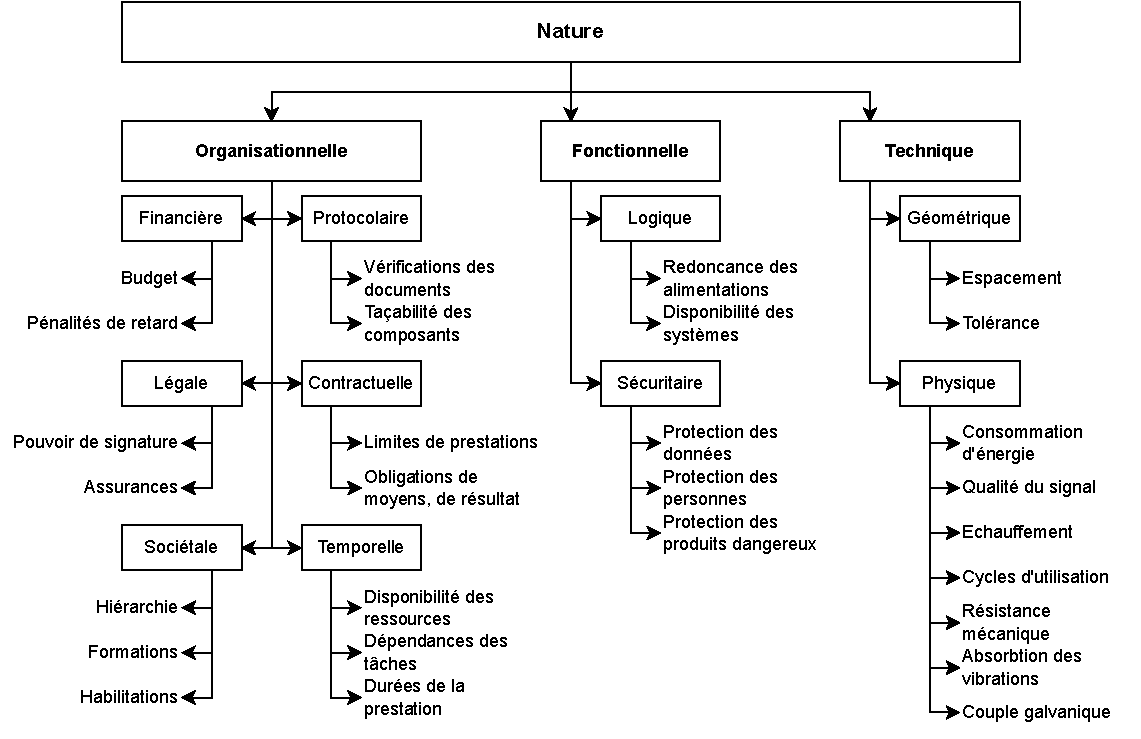
\includegraphics[width=.9\linewidth]{./svg/taxonomie.pdf}
\caption{\label{fig:orga687d35}Hierarchie des contraintes}
\end{figure}

Justifier le besoin d'une "méthode de rédaction générique".
\subsubsection{{\bfseries\sffamily TODO} Contraintes dans l’électrotechnique}
\label{sec:org490812c}
Présenter les contraintes spécifiques aux systèmes électriques (IEC 60364, NF C15-100, sécurité, synchronisation).  
Donner un exemple concret (poste de transformation).
\subsection{Cycle de vie des contraintes}
\label{sec:orgfb7d5af}
\subsubsection{{\bfseries\sffamily TODO} Exercice des contraintes}
\label{sec:org9cb545d}
\todo[inline]{expliciter le cycle de vie des contraintes}
Dans l'industrie de la construction, les parties prenantes se coordonnent dans la réponse à des exigences exprimées. Cette gestion des éxigences vise l'atteinte des objectifs du client en respect des contraintes légales, réglementaires et normatives.

\begin{quote}
Les exigences sont déterminées à partir des besoins des parties prenantes et des contraintes comme les conditions d’utilisation, les ressources et la législation. -- NF EN 60300-1:2014\autocite{GestionSureteFonctionnement2014}
\end{quote}

La relation entre éxigences et contraintes est représentée par la \ref{fig:orgd198976}. Ainsi, une exigence est une spécification d'un besoin tenant compte des contraintes du domaine d'étude. Cependant, la limite est souvent floue entre un besoin, une contrainte et une exigence. Les professionnels de la construction ont donc tendance à les mélanger.

\begin{figure}[htbp]
\centering
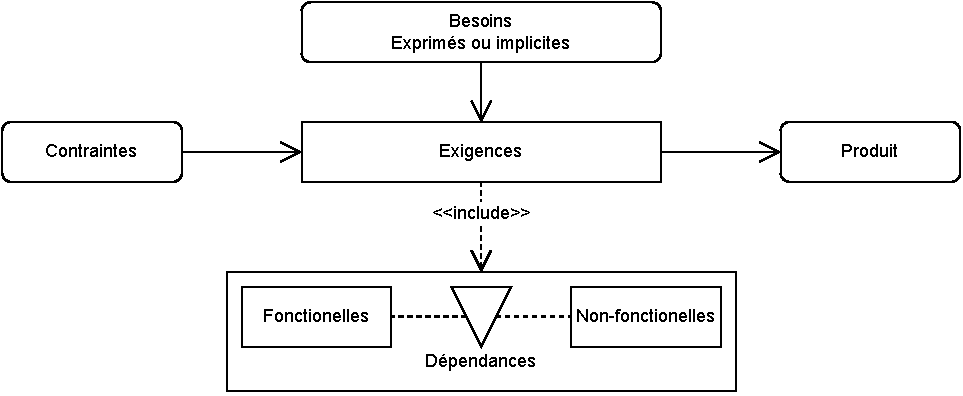
\includegraphics[width=.9\linewidth]{./svg/relation-contraintes-exigences.pdf}
\caption{\label{fig:orgd198976}La relation entre contraintes et exigences selont l'ISO 60300-1\autocite{GestionSureteFonctionnement2014}}
\end{figure}

Une matrice de traçabilité des exigences est employé pour réalisé le suivi des exigences.

Elle se matérialise par un tableau ou un document qui relie les exigences d'un projet aux livrables, tâches, jalons ou tests qui les satisfont. Son objectif principal est de garantir que toutes les exigences sont couvertes par les plans du projet et qu'aucun besoin n'est négligé. Elle permet également de vérifier l'impact des modifications d'exigences, facilitant la gestion des changements.

Élaboration de la matrice :
\begin{enumerate}
\item Collecte des exigences : rassembler toutes les exigences du projet, qu'elles proviennent du cahier des charges, des réunions avec les parties prenantes, d'autres documents de projet ainsi que des textes institutionnels applicables.
\item Identification des livrables : Listez tous les livrables du projet, y compris les rapports, les documents, le code source, les schémas, les maquettes numériques, les plans, etc.
\item Préparer la matrice : la première colonne source les exigences et la première ligne source les livrables. La première cellule (eg. A1:A1) est laissée vide.
\item Affecter les livrables aux exigences : Une croix est inscrite à l'intersection de chaque exigence devant être respectée ou vérifiée par un livrable. Un livrable peut être affecté à plusieurs exigences et une exigence peut nécessiter plusieurs livrables pour être vérifié. Cette étape nécessite une compréhension approfondie du projet et une collaboration étroite avec les équipes techniques.
\end{enumerate}

Utilisation de la matrice :
\begin{itemize}
\item Vérification de la couverture des exigences : la matrice permet de s'assurer que chaque exigence est adressée par au moins un livrable, réduisant ainsi le risque d'omissions.
\item Gestion des changements : Lorsque des modifications sont apportées à une exigence, la matrice facilite l'identification des livrables impactés, aidant à évaluer l'ampleur et l'impact du changement sur le projet.
\item Communication avec les parties prenantes : La matrice fournit une vue d'ensemble claire qui peut être utilisée pour communiquer l'avancement du projet et la manière dont les exigences sont satisfaites, renforçant la confiance des parties prenantes.
\item Facilitation des tests : En liant les exigences aux cas de test, la matrice aide à s'assurer que tous les aspects du système sont correctement testés, contribuant à la qualité du produit final.
\end{itemize}

La matrice de traçabilité des exigences est un document vivant qui \textbf{doit être régulièrement mis à jour tout au long du projet}. Les ajouts, les suppressions ou les modifications d'exigences, ainsi que l'évolution des plans de livrables, doivent être reflétés dans la matrice pour maintenir sa précision et sa pertinence.
Elle est employée en complément d'une liste des documents exécutés par le prestataire.

La nature de sa composition s'apparente à une table de jonction d'une base de donnée relationnelle tel que pourrait définir, sous forme de MLD la figure \ref{fig:orgee7ec83}.

\begin{figure}[htbp]
\centering
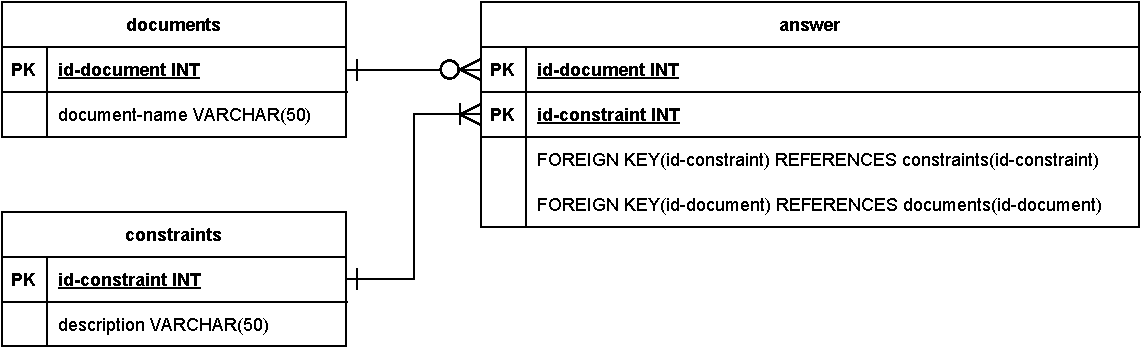
\includegraphics[width=.9\linewidth]{./svg/db-exigences-lde.pdf}
\caption{\label{fig:orgee7ec83}MLD - Association des éxigences aux livrables}
\end{figure}
\subsection{Impact sur la charge cognitive}
\label{sec:orgd7a8f4b}
\subsubsection{{\bfseries\sffamily TODO} Médiums et volumétrie}
\label{sec:org47f8cc4}
\todo[inline]{expliciter la problèmatique : taille du corpus, diversité des sources, silotage des rédactions (pas de travail conjoint entre les organismes producteurs de contraintes), difficulté d'en connaitre, etc.}
Sources, origines et finalités

Brevets, Normes, Législation, Contrats, Jurisprudences\ldots{}

Volume conséquent => faire un compte du nombre de pages par domaine pour illustrer la problématique.

\begin{figure}[htbp]
\centering
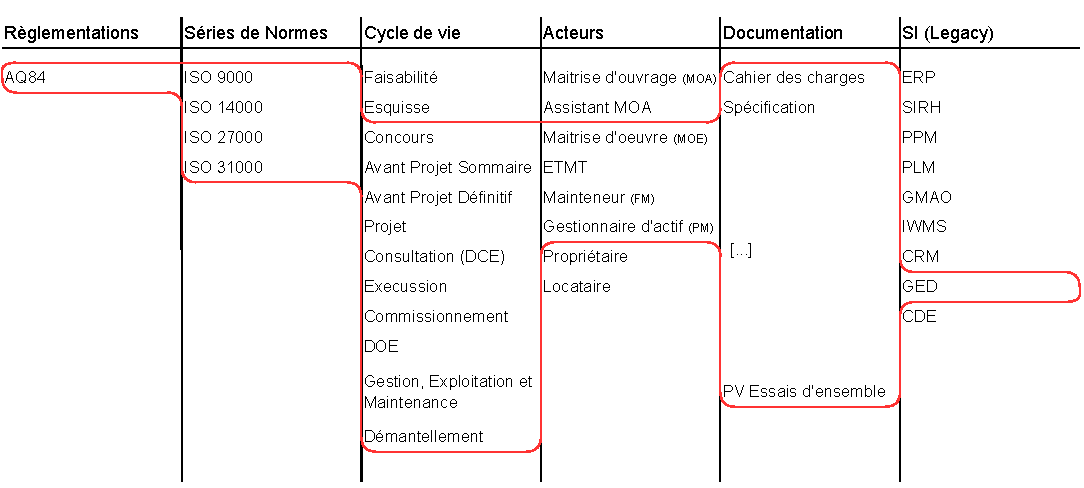
\includegraphics[width=.9\linewidth]{./svg/360-view-engineering-environment.pdf}
\caption{\label{fig:org9c2c7b2}Proposition de représentation des environnements de contraintes}
\end{figure}

\todo[inline]{voie de recherche possible : création d'un service de fourniture de contrainte standardisé et unifié appelable via des requettes API}
\subsubsection{{\bfseries\sffamily TODO} Environnement multi-acteur}
\label{sec:orgf5c4e06}
Décrire la multiplicité des acteurs et la complexité des interactions.  
Présenter les risques d’asymétrie d’information et la charge cognitive associée.  
Relier à la théorie de la cognition distribuée (Hutchins, 1995).
\subsection{Cadre de travail}
\label{sec:orgcead265}
\todo[inline]{on pose ici les 3 composantes du projet de recherche lié aux contraintes}
Les contraintes étant centraux à la caractérisation d'un ouvrage, il convient de définir un cadre de travail rigoureux permettant leurs manipulation.

Ce cadre doit poséder à minimum 3 composantes :
\begin{itemize}
\item Modélisation : formulation, négociation et amélioration des contraintes ;
\item Résolution : vérification de l'espace de solution, contrôle automatisé du respect des contraintes ;
\item Préservation : suivi des évolutions, association contextuelle, recherche d'information, etc.
\end{itemize}

Modélisation des contraintes : c’est l’activité de formulation et de négociation des contraintes en amont et au fil du projet. Il s’agit d’identifier clairement toutes les contraintes pertinentes (contextuelles, contractuelles, techniques…), de les exprimer de façon non ambiguë (rédaction dans le cahier des charges, spécifications, notes de calcul, modèles \protect\hyperlink{gls-18}{\label{gls-18-use-2}UML}, etc.) et de s’assurer qu’elles sont comprises et acceptées par les parties prenantes. La modélisation inclut éventuellement la négociation de certaines contraintes : par exemple discuter d’une tolérance plus large si une exigence s’avère trop restrictive par rapport au coût, ou reformuler un besoin implicite en exigences explicites testables. Un bon modèle de contraintes se veut complet, traçable et partagé par tous, servant de référence commune.

Résolution des contraintes : ce volet recouvre la satisfaction effective des contraintes lors de la recherche de solution et de la réalisation du projet. Il s’agit d’abord de procéder à la résolution du problème en trouvant un espace de solution qui respecte l’ensemble des contraintes identifiées – en d’autres termes, vérifier qu’il existe au moins une solution faisable (vérification de la non-surcontrainte). Ensuite, on s’assure du juste niveau de contrainte : éviter d’ajouter des contraintes inutiles ou trop sévères qui surcontraindraient le projet par rapport au besoin réel. Cela implique une optimisation : assez de contraintes pour rencontrer le besoin et les objectifs, mais pas au point d’éliminer des solutions viables ou d’alourdir le projet inutilement. Enfin, ce volet inclut la vérification du respect des contraintes tout au long des études et de l’exécution – par des revues de conception, des simulations, des prototypes ou des tests. Chaque décision technique ou modification doit être évaluée au prisme des contraintes : si une solution envisagée viole une contrainte (par exemple une charge dépassant la contrainte de poids maximal), il faut soit l’ajuster, soit envisager de redéfinir la contrainte si cela est justifié et approuvé.

Préservation des contraintes (capitalisation) : au-delà du respect ponctuel, il est crucial de préserver la mémoire des contraintes du projet et de leur évolution. Ce troisième volet consiste à historiser et documenter les contraintes, leurs justifications d’origine, et les éventuelles modifications apportées en cours de route (assouplissements, ajouts, suppressions), de sorte que l’on sache à tout moment pourquoi telle contrainte a été posée et pourquoi tel choix de conception a été fait en conséquence. Cette traçabilité garantit la cohérence du projet sur la durée et facilite la maintenance ou les évolutions futures. Par exemple, conserver dans un registre ou une base de connaissance le raisonnement ayant conduit à une contrainte particulière (issue d’une norme, d’un retour d’expérience, d’une demande client spécifique…) permettra, des années plus tard, à un nouvel intervenant de comprendre le rationnel de conception. La préservation des contraintes et de leur historique de négociation contribue ainsi à une gestion de configuration rigoureuse et à l’amélioration continue du référentiel de conception de l’entreprise.

En conjuguant ces trois dimensions, on dote la notion de contrainte d’un véritable cadre de gestion sur le projet en respectant la définition \ref{orgd37e898}.
\subsubsection{{\bfseries\sffamily TODO} Méthodes de traitement}
\label{sec:orgca4ced3}
Langage naturel :
\begin{itemize}
\item Rédaction
\item Affectation (par des tableaux et matrices)
\item Relecture (sur la base de listes à puces, checklist)
\item Simulations (éventuellement mais loop sur rapport produit)
\item Model checking : vérification exhaustive d'états finis, non systématique à date et loop sur rapport produit
\end{itemize}
\subsection{Conclusion}
\label{sec:org0b24503}
\clearpage
\section{Proposition (80p)}
\label{sec:org8b0fa9d}
\subsection{Méthodologie de conception}
\label{sec:org57edf46}
\subsubsection{{\bfseries\sffamily TODO} Conception orientée par le domaine}
\label{sec:org92a6666}

\subsubsection{{\bfseries\sffamily TODO} Conception centrée utilisateur}
\label{sec:org83a1c50}
Décrire la démarche UCD (ISO 9241-210) appliquée au projet : itérations, co-design, implication des acteurs.
\subsubsection{{\bfseries\sffamily TODO} Adaptation des méthodes agiles}
\label{sec:orgfb40dcb}
Présenter l’articulation entre Scrum et les processus de modélisation.  
Identifier les correspondances : sprint ↔ phase, backlog ↔ liste de contraintes.
\subsubsection{{\bfseries\sffamily TODO} Développement piloté par les comportements}
\label{sec:org1917700}
Décrire les modalités d’évaluation :  
\begin{itemize}
\item Tests utilisateurs : SUS, NASA-TLX
\item Mesures : temps, précision, charge cognitive
\item Outils : enregistrements, questionnaires, logs.
\end{itemize}
\subsection{Architecture logicielle}
\label{sec:orga880ac0}
\subsubsection{Choix technologiques}
\label{sec:orge734e58}
\subsubsection{Modules principaux}
\label{sec:org3517ccd}
\subsubsection{Tests unitaires et d'intégration}
\label{sec:org44d24b0}
\subsection{Conclusion}
\label{sec:orgfd31bba}
\clearpage
\section{Protocol expérimental (15p)}
\label{sec:orgf729861}
\subsection{Fondements méthodologiques}
\label{sec:org6a891ba}
Ce protocole s’appuie sur deux cadres théoriques principaux :
\begin{itemize}
\item \textbf{Cognitive Load Theory} (Sweller, 1988) — la performance dépend du niveau de charge cognitive induite par l’interface et la tâche.
\item \textbf{Neuroergonomie} (Parasuraman \& Rizzo, 2007) — mesure de l’efficience cérébrale et physiologique de l’interaction homme-machine.
\end{itemize}

Objectif général : évaluer l’impact du prototype QuickMotion sur la rapidité et la fiabilité de la réalisation des tâches par rapport à une interface de référence.
\subsection{Questions de recherche}
\label{sec:orgf45744c}
\begin{itemize}
\item \textbf{\textbf{Q1 :}} Le prototype permet-il de résoudre les problèmes plus rapidement ?
\item \textbf{\textbf{Q2 :}} Le prototype permet-il de réduire le nombre d’erreurs ?
\end{itemize}
\subsection{Périmètre des essais}
\label{sec:org8c05ab9}
\subsubsection{Constitution des groupes de participants}
\label{sec:org95c6a4c}
\begin{table}[htbp]
\caption{\label{tab:orgb426b9c}Constitution des groupes de test et des finalités recherchées}
\centering
\begin{tabular}{llrlll}
 & Population & Taille & Localisation & Phase & Finalités\\
\hline
G1 & Équipe de recherche & 3 & Laboratoire & Concept & Validation conceptuelle\\
G2 & Membres du laboratoire & 5 & Laboratoire & Pilote & Ajustement du protocole\\
G3 & Groupe contrôle & 8 & Locaux du partenaire & Pilote & Calibrage des essais\\
G4 & Groupe caractérisé & 24 pers. (2 conditions) → 48 obs. & Centre de formation & Principale & Objectiver les données\\
G5 & Plateforme libre d’accès & Variable (≥500 jusqu’à >20k) & En ligne & Test A/B & Représentativité statistique\\
\end{tabular}
\end{table}

Principes de planification
\begin{itemize}
\item \textbf{G1 → G3} : conception et calibration des instruments.
\item \textbf{G4} : étude principale en plan intra-sujets (chaque participant teste les deux interfaces, ordre contrebalancé).
\item \textbf{G5} : étude à large échelle, randomisation 1:1 (version A/B), analyse séquentielle selon le nombre effectif de participants.
\end{itemize}
\subsubsection{Données à collecter}
\label{sec:orge77e36d}
\begin{table}[htbp]
\caption{\label{tab:org818a5ba}Synthèse des données collectées}
\centering
\begin{tabular}{llllll}
ID & Caractéristique & Mesure & Moyen de collecte & Groupes & Question\\
\hline
D1 & Performance & Temps de complétion & Chronométrie embarquée & G1–G5 & Q1\\
D2 & Performance & Nombre d’erreurs & Compteur d’événements & G1–G5 & Q2\\
D3 & Utilisabilité & Navigation & Changement d’écran & G1–G5 & —\\
D4 & Utilisabilité & Nombre de clics & Logger embarqué & G1–G5 & —\\
D5 & Utilisabilité & Entrées clavier & Logger embarqué & G1–G5 & —\\
D6 & Physiologique & Fréquence cardiaque & Montre connectée Redmi Watch 5 Lite & G1–G4 & —\\
D7 & Physiologique & SpO₂ & Montre connectée & G1–G4 & —\\
D8 & Physiologique & Mouvements oculaires & Webcam + eye-tracker logiciel & G1–G4 & —\\
D9 & Physiologique & Ondes cérébrales (EEG, optionnel) & Casque EEG léger & G3–G4 & —\\
D10 & Perceptuelle & Charge subjective & SWAT (Reid \& Nygren, 1988) & G1–G5 & —\\
D11 & Perceptuelle & Charge de tâche & NASA-TLX (Hart \& Staveland, 1988) & G1–G5 & —\\
D12 & Perceptuelle & Acceptabilité & SUS ou UMUX-Lite & G1–G5 & —\\
D13 & Qualitative & Stratégie, obstacles, raisons & Entretiens semi-directifs & G1–G3 & —\\
\end{tabular}
\end{table}
\subsubsection{Instruments et logiciels}
\label{sec:org3ab2114}
\begin{itemize}
\item \textbf{\textbf{Montre connectée :}} Redmi Watch 5 Lite (\textasciitilde{}40 €/u)
\item \textbf{\textbf{Webcam :}} HD ≥1080p, 30 fps
\item \textbf{\textbf{Logiciels :}}
\begin{itemize}
\item \textbf{Eye-tracking :} logiciel libre de suivi du regard (par ex. \texttt{WebGazer.js} ou \texttt{OpenFace})
\item \textbf{Randomisation A/B :} module serveur interne (tirage pseudo-aléatoire 1:1)
\item \textbf{Questionnaires :} formulaires intégrés (Google Forms ou LimeSurvey)
\item \textbf{Agrégation :} Prometheus
\end{itemize}
\end{itemize}
\subsection{Analyse statistique}
\label{sec:org5e4239a}
Hypothèses
\begin{itemize}
\item H₀ : aucune différence entre A et B.
\item H₁ : le prototype (B) améliore les performances (temps, erreurs).
\end{itemize}

Tests
\begin{itemize}
\item \textbf{Temps de complétion} → Wilcoxon rangs signés (intra) ou Mann-Whitney (inter).
\item \textbf{Nombre d’erreurs} → McNemar (intra) ou χ²/Fisher (inter).
\item \textbf{Scores questionnaires} → tests non paramétriques équivalents.
\end{itemize}

Indices
\begin{itemize}
\item Effet moyen : \textbf{Cohen’s d} ou \textbf{r de rangs}.
\item Intervalle de confiance 95 \% pour chaque différence.
\end{itemize}
\subsubsection{Seuils statistiques}
\label{sec:orgddad478}
Paramètres
\begin{itemize}
\item α = 0.05 ; puissance = 0.80 ; allocation 1:1.
\item Unité d’analyse : utilisateur unique.
\end{itemize}

Interprétation selon taille effective (N\_total)
\begin{table}[htbp]
\caption{MDE (Minimal Detectable Effect) selon taille d’échantillon}
\centering
\begin{tabular}{lllll}
N\_total & n/bras & MDE@pA=20\% & MDE@pA=50\% & Interprétation\\
\hline
200 & 100 & 26.0 pp & 26.7 pp & Détecte seulement gros effets\\
500 & 250 & 15.8 pp & 17.4 pp & Effets massifs\\
1,000 & 500 & 10.9 pp & 12.4 pp & Gros effets\\
2,000 & 1,000 & 7.5 pp & 8.8 pp & Effets moyens\\
4,000 & 2,000 & 5.2 pp & 6.2 pp & Effets modestes\\
10,000 & 5,000 & 3.3 pp & 4.0 pp & Effets faibles\\
20,000 & 10,000 & 2.3 pp & 2.8 pp & Petits effets\\
100,000 & 50,000 & 1.0 pp & 1.25 pp & Très petits effets\\
\end{tabular}
\end{table}

Ces seuils déterminent les limites des interprétations réalisables au regard du nombre de participants constituant le groupe G5.

Lecture a posteriori
\begin{enumerate}
\item Calculer \(\hat{p}_A, \hat{p}_B, \Delta = \hat{p}_B - \hat{p}_A\)
\item Estimer IC95 \% (méthode de Newcombe)
\item Interpréter :
\begin{itemize}
\item Si 0 ∉ IC95 \% et |Δ| ≥ MDE → effet établi.
\item Si 0 ∉ IC95 \% et |Δ| < MDE → effet réel mais faible.
\item Si 0 ∈ IC95 \% → résultat inconclusif.
\end{itemize}
\item Reporter toujours IC95 \% et borne supérieure de Δ.
\end{enumerate}

Règles d’arrêt
\begin{itemize}
\item \textbf{Succès} : premier palier où 0 ∉ IC95 \% et |Δ| ≥ MDE.
\item \textbf{Futilité} : |Δ| + marge plausible < MDE → arrêt.
\item \textbf{Sécurité} : arrêt si indicateur d’erreur ou fatigue dépasse seuil.
\end{itemize}
\subsection{Organisation des essais}
\label{sec:org2495de2}
\subsubsection{Contrôles et biais anticipés}
\label{sec:org8316ff8}
\begin{itemize}
\item \textbf{Randomisation / contrebalancement :} neutraliser effets d’ordre.
\item \textbf{Masquage :} expérimentateur aveugle à la version présentée.
\item \textbf{Effet observateur / Hawthorne :} temps d’adaptation avant mesure, consignes neutres.
\item \textbf{Demand characteristics :} hypothèses dissimulées.
\item \textbf{Filtrage aberrants :} sessions <5e ou >95e percentile, abandons.
\item \textbf{Biais évaluateur :} double codage et audits croisés.
\item \textbf{Attrition :} compensation équitable et sessions courtes.
\item \textbf{Contrôle matériel :} même environnement, machine, luminosité.
\item \textbf{Familiarisation :} un essai non mesuré.
\end{itemize}
\subsubsection{Déroulement expérimental}
\label{sec:org2a32277}
\begin{itemize}
\item Phase G1–G3 : validation des tâches, étalonnage des instruments, estimation des variances.
\item Phase G4 : session en plan croisé AB/BA (ordre contrebalancé).  
1 essai d’entraînement non mesuré avant chaque condition.
\item Phase G5 : randomisation automatique des utilisateurs vers A ou B.  
Données loguées serveur (horodatage, succès, erreurs, métriques comportementales).
\end{itemize}
\subsection{Synthèse et limites}
\label{sec:orgdb5b4b1}
\begin{table}[htbp]
\caption{\label{tab:org533e867}Réponses attendues}
\centering
\begin{tabular}{llll}
Question & Indicateur principal & Réponse attendue & Test prévu\\
\hline
Q1 & Temps de complétion & B < A & Wilcoxon ou Mann-Whitney\\
Q2 & Nombre d’erreurs & B < A & McNemar ou χ²/Fisher\\
— & Charge perçue (NASA-TLX) & B < A & Test non paramétrique\\
— & Acceptabilité (SUS) & B > A & Test non paramétrique\\
\end{tabular}
\end{table}

Limites prévues
\begin{itemize}
\item Variabilité individuelle élevée (temps, stress) → moyennes pondérées ou normalisation intra-sujet.
\item Données physiologiques sensibles aux artefacts → exclusion si signal <70 \% qualité.
\item Étude A/B soumise à biais d’échantillon si recrutement libre.
\end{itemize}

Perspective
Les résultats des phases G1–G4 permettront d’ajuster le prototype et d’estimer les paramètres statistiques réels (écarts types, proportions d’erreurs).  
Ces estimations alimenteront le calcul de puissance pour G5 et orienteront la décision de passage à une expérimentation de grande échelle ou à une version stable du prototype.
\subsection{Conclusion}
\label{sec:org3448635}
\clearpage
\section{Validation expérimentale (50p)}
\label{sec:org7a9c9fa}
\subsection{Cas d'étude 1 :}
\label{sec:orge9aa253}
\subsubsection{{\bfseries\sffamily TODO} Présentation du cas d’étude}
\label{sec:org21c2507}
Décrire le contexte du poste de transformation ferroviaire.  
Lister les acteurs impliqués, leurs rôles et contraintes spécifiques.
\subsubsection{{\bfseries\sffamily TODO} Déploiement du prototype}
\label{sec:orge91f575}
Décrire l’architecture logicielle : pipeline CNL → Graph → Solveur → IHM.  
Identifier les flux, les technologies, et le protocole d’observation.
\subsubsection{{\bfseries\sffamily TODO} Collecte et analyse des données}
\label{sec:org1abac4f}
Présenter la méthodologie d’analyse mixte (quantitative et qualitative).  
Décrire les indicateurs de performance et les observations comportementales.
\subsubsection{{\bfseries\sffamily TODO} Validation expérimentale}
\label{sec:org74a9578}
Présenter les résultats et la discussion.  
Évaluer l’efficacité du prototype : charge cognitive réduite, détection d’incohérences, traçabilité accrue.
\subsection{Cas d'étude 2 :}
\label{sec:orga306e39}
\subsubsection{{\bfseries\sffamily TODO} Présentation du cas d’étude}
\label{sec:org84526f9}
Décrire le contexte du poste de transformation ferroviaire.  
Lister les acteurs impliqués, leurs rôles et contraintes spécifiques.
\subsubsection{{\bfseries\sffamily TODO} Déploiement du prototype}
\label{sec:org19906a0}
Décrire l’architecture logicielle : pipeline CNL → Graph → Solveur → IHM.  
Identifier les flux, les technologies, et le protocole d’observation.
\subsubsection{{\bfseries\sffamily TODO} Collecte et analyse des données}
\label{sec:orge10cc0e}
Présenter la méthodologie d’analyse mixte (quantitative et qualitative).  
Décrire les indicateurs de performance et les observations comportementales.
\subsubsection{{\bfseries\sffamily TODO} Validation expérimentale}
\label{sec:orgb3b1701}
Présenter les résultats et la discussion.  
Évaluer l’efficacité du prototype : charge cognitive réduite, détection d’incohérences, traçabilité accrue.
\subsection{Cas d'étude 3 :}
\label{sec:orgaade1af}
\subsubsection{{\bfseries\sffamily TODO} Présentation du cas d’étude}
\label{sec:org2d4e361}
Décrire le contexte du poste de transformation ferroviaire.  
Lister les acteurs impliqués, leurs rôles et contraintes spécifiques.
\subsubsection{{\bfseries\sffamily TODO} Déploiement du prototype}
\label{sec:org795f976}
Décrire l’architecture logicielle : pipeline CNL → Graph → Solveur → IHM.  
Identifier les flux, les technologies, et le protocole d’observation.
\subsubsection{{\bfseries\sffamily TODO} Collecte et analyse des données}
\label{sec:org177a415}
Présenter la méthodologie d’analyse mixte (quantitative et qualitative).  
Décrire les indicateurs de performance et les observations comportementales.
\subsubsection{{\bfseries\sffamily TODO} Validation expérimentale}
\label{sec:org149ca03}
Présenter les résultats et la discussion.  
Évaluer l’efficacité du prototype : charge cognitive réduite, détection d’incohérences, traçabilité accrue.
\subsection{Analyse des résultats}
\label{sec:org3455003}
\subsubsection{Descriptions}
\label{sec:org21b7c02}

\begin{itemize}
\item Analyse de contenu détaillée : En appliquant la méthode d’analyse de contenu au corpus (selon Bardin, par exemple), on poursuit après le codage avec le comptage et la description des thèmes identifiés. Il s’agit de quantifier la fréquence d’apparition de chaque type de problème ou de commentaire pour évaluer leur importance relative. \url{https://journals.openedition.org/ripes/2996\#:\~:text=n\%C3\%A9gociation\%20entre\%20ses\%20croyances\%20propres,Ces\%20derni\%C3\%A8res\%20peuvent}
\end{itemize}
\subsubsection{Interprétations}
\label{sec:org543fcaa}

\begin{itemize}
\item Outils d’analyse qualitative : On peut recourir à des outils informatiques pour faciliter le traitement des données textuelles (par ex. le logiciel RQDA sous R, comme dans l’étude de Chartofylaka et al. \url{https://journals.openedition.org/ripes/2996\#:\~:text=n\%C3\%A9gociation\%20entre\%20ses\%20croyances\%20propres,Ces\%20derni\%C3\%A8res\%20peuvent}, ou un logiciel d’analyse qualitative tel que NVivo, Atlas.ti, etc.). Ces outils permettent de coder des segments de texte, de regrouper par thème et d’extraire toutes les citations liées à un thème donné, ce qui accélère l’analyse tout en la rendant traçable.
\item Utilisation du schéma de Barnum : D’après Barnum (domaine de l’ergonomie IHM), une bonne triangulation en évaluation d’interface consiste à comparer trois volets : (1) les mesures de performance objectives, (2) les mesures subjectives (questionnaires, interviews) et (3) la liste des problèmes d’utilisabilité identifiés \url{https://cs4760.csl.mtu.edu/2020/lectures/usability-testing/\#:\~:text=Barnum\%20suggests\%20triangulation\%20analysis\%20which,is\%20a\%20comparison\%20of}.
\item Illustration par des exemples : Pour rendre la description des résultats vivante et compréhensible, on prendra soin d’intégrer dans le rapport final des exemples concrets tirés des données qualitatives.
\end{itemize}

\begin{table}[htbp]
\caption{\label{tab:orgbbf0330}Matrice de validation expérimentale — IHM écologique et gestion des contraintes}
\centering
\begin{tabular}{lllll}
ID & Variable indépendante (manipulée) & Variable dépendante (mesurée) & Type d’évaluation & Instruments / métriques\\
\hline
 &  &  &  & \\
 &  &  &  & \\
\end{tabular}
\end{table}
\subsection{Conclusion}
\label{sec:org68da532}
\clearpage
\section{Discussion et perspectives (15p)}
\label{sec:org84af989}
\subsection{Analyse des contributions}
\label{sec:org34b0921}
\subsubsection{Contributions théoriques}
\label{sec:org72f6264}
\subsubsection{Contributions méthodologiques}
\label{sec:org6bd6c47}
\begin{itemize}
\item Protocole d’évaluation centré utilisateur
\end{itemize}
\subsubsection{Contributions pratiques}
\label{sec:org71d6781}
\begin{itemize}
\item Modèle d’IHM écologique sensible aux contraintes
\item Prototype validé en environnement réel
\end{itemize}
\subsection{Limites et recommandations}
\label{sec:org82e1f40}
\subsubsection{Limites théoriques}
\label{sec:orga685cea}
\subsubsection{Limites pratiques}
\label{sec:orgadf4cf1}
\subsubsection{Recommandations}
\label{sec:orgdbe115d}
\subsection{Perspectives et opportunités}
\label{sec:org90a87ce}
\subsubsection{Extensions théoriques}
\label{sec:orgfd36fe0}

\begin{figure}[htbp]
\centering
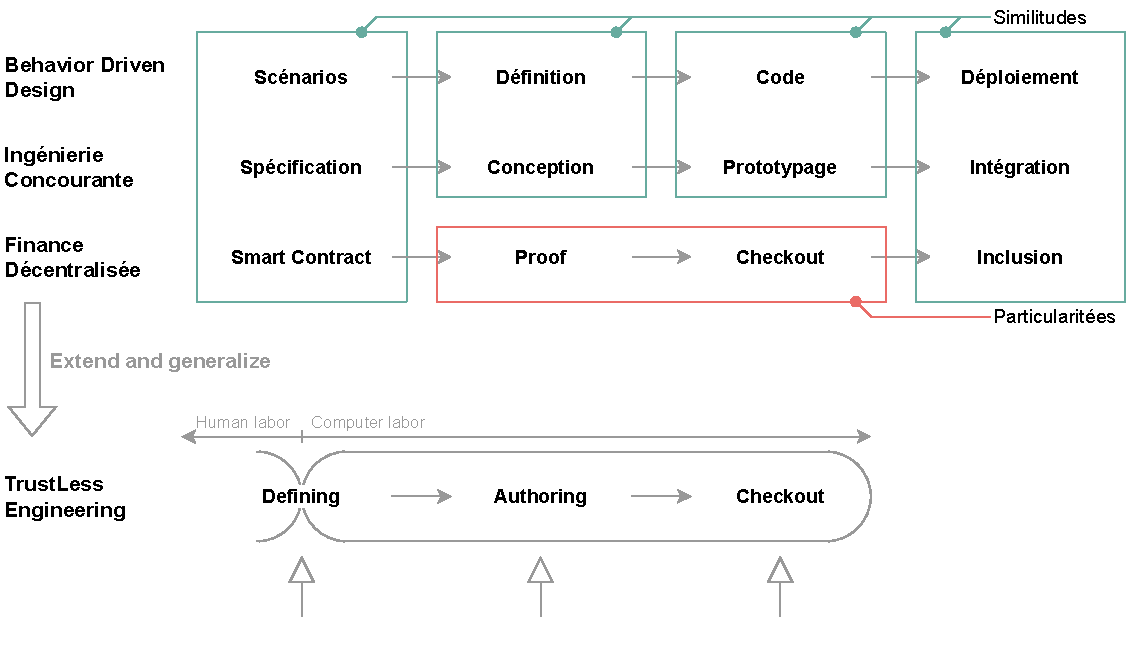
\includegraphics[width=.9\linewidth]{./svg/long-term-goal.pdf}
\caption{\label{fig:orgb49374e}Vers une ingénierie sans confiance ?}
\end{figure}
\subsubsection{Opportunités de recherche}
\label{sec:orgacf2593}
\begin{itemize}
\item IA
\item Block Chain
\item Solveur de contrainte
\item Analyse statique du texte (NLP)
\item Intégration dynamique d'ontologies métiers
\end{itemize}
\subsubsection{Transfert technologique}
\label{sec:orgc9545a9}
à d'autres industries,
à la fabrique de la norme et de la législation\ldots{}
\subsection{Impact scientifique et industriel}
\label{sec:org056b238}
\subsubsection{Impact sur la recherche}
\label{sec:org8030f15}
\subsubsection{Impact industriel}
\label{sec:org5e541c0}
\subsubsection{Impact sociétal}
\label{sec:org66b2256}
Discuter de la faisabilité et des implications de la refonte de la filière.
\clearpage
\section{Conclusion générale (10p)}
\label{sec:orga2a2068}
Synthèse des contributions

Contribution théorique majeure

Innovation méthodologique

Validation expérimentale

Réponse à la question principale

Réponse à la questions secondaires

Perspectives d'avenir


\begin{quote}
{[}!Info] Commentaire prospectif sur l'ouvrage et ses conclusions
\end{quote}

Espérer une évolution des plateformes d'accès aux normes (cobaz) pour simplifier la configuration des environnements de travail (NF EN etc. et gestion des exigences)

L'avenir, un terrain fertile pour l'ingénierie intégrée ?

Les futures ruptures technologiques (?)
\clearpage

\clearpage
\section{Références du document}
\label{sec:org48cec11}
\subsection{Liste des figures}
\label{sec:org5d77b04}
\renewcommand{\listfigurename}{\vspace{-2em}}
\listoffigures
\subsection{Liste des tableaux}
\label{sec:orgaf488bf}
\renewcommand{\listtablename}{\vspace{-2em}}
\listoftables
\subsection{Liste des codes sources}
\label{sec:org645d339}
\renewcommand{\lstlistingname}{\vspace{-2em}}
\lstlistoflistings
\subsection{Liste des glosses}
\label{sec:org669c655}
\begin{multicols}{2}\small{

}\end{multicols}
\subsection{Liste des acronymes}
\label{sec:org1287467}

\textbf{B}

\textbf{\hypertarget{gls-78}{BPMN}}\hspace*{1em}Business Process Model and Notation\hspace*{.5em}\pageref{gls-20-use-1}

\textbf{\hypertarget{gls-73}{BOS}}\hspace*{1em}Building Operating System\hspace*{.5em}\pageref{gls-6-use-1}, \pageref{gls-6-use-2}

\textbf{\hypertarget{gls-70}{BIS}}\hspace*{1em}Building Information System\hspace*{.5em}\pageref{gls-5-use-1}, \pageref{gls-5-use-2}

\textbf{\hypertarget{gls-69}{BIM}}\hspace*{1em}Building Information Modeling\hspace*{.5em}\pageref{gls-1-use-1}, \pageref{gls-1-use-2}, \pageref{gls-1-use-3}, \pageref{gls-1-use-4}, \pageref{gls-1-use-5}, \pageref{gls-1-use-6}, \pageref{gls-1-use-7}, \pageref{gls-1-use-8}, \pageref{gls-1-use-9}, \pageref{gls-1-use-10}, \pageref{gls-1-use-11}

\textbf{E}

\textbf{\hypertarget{gls-151}{ETMT}}\hspace*{1em}Entreprise Titulaire d'un Marché de Travaux\hspace*{.5em}\pageref{gls-11-use-1}

\textbf{G}

\textbf{\hypertarget{gls-176}{GTC}}\hspace*{1em}Gestion Technique Centralisée\hspace*{.5em}\pageref{gls-13-use-1}

\textbf{\hypertarget{gls-177}{GTB}}\hspace*{1em}Gestion Technique du Bâtiment\hspace*{.5em}\pageref{gls-12-use-1}

\textbf{\hypertarget{gls-169}{GED}}\hspace*{1em}Gestion Electronique des Documents\hspace*{.5em}\pageref{gls-7-use-1}, \pageref{gls-7-use-2}, \pageref{gls-7-use-3}, \pageref{gls-7-use-4}, \pageref{gls-7-use-5}

\textbf{I}

\textbf{\hypertarget{gls-194}{IoT}}\hspace*{1em}Internet of Things\hspace*{.5em}\pageref{gls-17-use-1}

\textbf{\hypertarget{gls-189}{IDS}}\hspace*{1em}Information Delivery Specifications\hspace*{.5em}\pageref{gls-8-use-1}

\textbf{\hypertarget{gls-186}{ICS}}\hspace*{1em}International Classification for Standards\hspace*{.5em}\pageref{gls-21-use-1}, \pageref{gls-21-use-2}, \pageref{gls-21-use-3}

\textbf{\hypertarget{gls-185}{ICE}}\hspace*{1em}Integrated Concurrent Engineering\hspace*{.5em}\pageref{gls-3-use-1}, \pageref{gls-3-use-2}, \pageref{gls-3-use-3}

\textbf{L}

\textbf{\hypertarget{gls-209}{LOIN}}\hspace*{1em}Level Of Information Need (ISO 19650)\hspace*{.5em}\pageref{gls-2-use-1}

\textbf{M}

\textbf{\hypertarget{gls-232}{MPLS}}\hspace*{1em}Multiprotocol Label Switching\hspace*{.5em}\pageref{gls-16-use-1}

\textbf{\hypertarget{gls-228}{MOE}}\hspace*{1em}Maitrise d'Œuvre\hspace*{.5em}\pageref{gls-10-use-1}

\textbf{\hypertarget{gls-225}{MOA}}\hspace*{1em}Maitrise d’OuvrAge\hspace*{.5em}\pageref{gls-9-use-1}

\textbf{S}

\textbf{\hypertarget{gls-332}{SysML}}\hspace*{1em}System Model Language\hspace*{.5em}\pageref{gls-19-use-1}

\textbf{\hypertarget{gls-305}{SCADA}}\hspace*{1em}Système de Contrôle et d'Acquisition de Données\hspace*{.5em}\pageref{gls-15-use-1}

\textbf{U}

\textbf{\hypertarget{gls-339}{UML}}\hspace*{1em}Unified Model Language\hspace*{.5em}\pageref{gls-18-use-1}, \pageref{gls-18-use-2}

\textbf{V}

\textbf{\hypertarget{gls-342}{VDI}}\hspace*{1em}Voix, Données et Images\hspace*{.5em}\pageref{gls-14-use-1}

\textbf{\hypertarget{gls-341}{VDC}}\hspace*{1em}Virtual Design and Construction\hspace*{.5em}\pageref{gls-4-use-1}, \pageref{gls-4-use-2}, \pageref{gls-4-use-3}, \pageref{gls-4-use-4}, \pageref{gls-4-use-5}

}\clearpage\end{multicols}
\section{Bibliographie}
\label{sec:orgb50d4b2}
\begin{multicols}{2}\small{
\printbibliography[heading=none]
}\clearpage\end{multicols}

\appendix
\section{Analyse des normes}
\label{sec:orga863a01}
\subsection{Introduction}
\label{sec:orgaa35096}
\subsection{Périmètre de l'étude}
\label{sec:orgb255d74}
L’étude se concentre sur les normes volontaires françaises (NF) référencées par AFNOR et publiées à la date de la collecte.
Le périmètre inclut toutes les normes relevant du domaine “Construction et urbanisme” selon la classification AFNOR Norm’Info.

Les normes ISO/IEC sont souvent transposées en normes NF (NF EN ISO, etc.)

AFNOR est le point d’entrée national reconnu par l’État pour la normalisation volontaire.

Les normes d’application obligatoire sont issues de ce corpus (via réglementations).

Par l'analyse des textes et de leurs métadonnées, nous tenterons de répondre aux questions suivantes :

\begin{itemize}
\item Q1 : Quelle est l’ampleur documentaire du corpus normatif applicable à l’industrie de la construction, mesurée en nombre de documents et en volume paginé ?
\item Q2 : La filière construction présente-t-elle une densité normative supérieure à celle d’autres secteurs industriels comparables, en termes de nombre de normes actives et de leur volumétrie documentaire ?
\item Q3 : Comment les textes normatifs se répartissent-ils entre les sous-domaines techniques, professions et spécialités représentatives de la filière construction, selon les descripteurs et indices de classement ?
\end{itemize}
\subsection{Méthodologie}
\label{sec:org305eb21}
\subsubsection{Cadre juridique}
\label{sec:orgfb3038e}
Il n'existe pas de base de données publiques recenssant l'ensemble des textes de normes et leurs métadonnées. Il convient donc de constituer cette base de donnée en collectant les informations publiquement accessibles.

Cette opération implique l'emplois du webscraping.

\begin{quote}
Le webscraping consiste à extraire automatiquement (to scrape : gratter), de manière massive des données d'un site web. -- INRAE\autocite{quesnevilleRecommandationsUsagesWebscraping2024}
\end{quote}

La légalité d'une telle opération semble parfois faire débat. (ref à ajouter)

Certains acteurs, notamment l'AFNOR, s'oppose à la fouille automatisée des texte que l'organisme fournis ainsi qu'à l'emploi de modèles d'intelligence artificielle sur ceux-ci tels que l'exprime ce paragraphe apposés en première page de couverture :
\begin{quote}
AFNOR, en tant que titulaire des droits d’auteur ou distributeur autorisé, s’oppose expressément à toute intégration, transmission ou absorption totale ou partielle du présent document par des moteurs ou algorithmes d’Intelligence Artificielle (IA). AFNOR s’oppose également à toute fouille de textes et de données ou création dérivée produite par une IA et basée sur le présent document.
\end{quote}

Cela dit, le Code de la propriété intellectuelle précise les modalités de copie et de reproduction des bases de données (Art. L342-3) et les droits de manipulation des textes dans un cadre de recherche scientifique (Art. L122-5 et L122-5-3)\autocite{CodeProprieteIntellectuelle} en précisant spécifiquement que :
\begin{quote}
Des copies ou reproductions numériques d'œuvres auxquelles il a été accédé de manière \textbf{licite} peuvent être réalisées \textbf{sans autorisation des auteurs} en vue de \textbf{fouilles de textes et de données} menées à bien aux seules fins de la recherche scientifique par les organismes de recherche [\ldots{}] ou pour leur compte et à leur demande par d'autres personnes, y compris dans le cadre d'un partenariat sans but lucratif avec des acteurs privés. -- Article L122-5-3\autocite{CodeProprieteIntellectuelle}
\end{quote}

L'exploration des textes publiés par l'AFNOR et obtenus de manière licite est donc autorisée.
\subsubsection{Données collectées}
\label{sec:org20bee2c}
Métadonnées accessibles publiquement via Norm’Info et Boutique AFNOR :
    Référence (ex : NF C15-100)
    Titre
    Date de publication
    Nombre de pages
    Codes International Classification for Standards
 (\protect\hyperlink{gls-21}{\label{gls-21-use-1}ICS})
    Indice de classement
    Domaine technique
    Commission de normalisation
\subsubsection{Protocole technique}
\label{sec:org188080b}
Méthode de collecte : Web scraping (à documenter)

Limite : seules les normes publiées et publiquement référencées sur le site marchand de l'AFNOR disponibles à la vente ou référencées, sont incluses.
\subsection{Méthodes d'analyse}
\label{sec:orgb1ec7ba}
Analyse descriptive :
    Nombre total de documents / pages
    Évolution temporelle des publications (si date disponible)

Analyse comparative :
    Densité normative dans la construction vs autres domaines AFNOR (en comparant les volumes \protect\hyperlink{gls-21}{\label{gls-21-use-2}ICS} sectoriels)

Analyse thématique / taxonomique :
    Catégorisation des normes par code \protect\hyperlink{gls-21}{\label{gls-21-use-3}ICS}, indice de classement, domaine technique
    Projection possible par métier : architecture, génie civil, thermique, électricité…

Outils recommandés : Python (pandas + matplotlib)
\subsection{Résultats obtenus}
\label{sec:orge08d938}
Cartographie de la norme dans la construction

Poids normatif par spécialité

Identification d’une sur-normativité éventuelle

Premiers indicateurs pour évaluer la « charge de la norme »
\subsection{Discussion et perspectives}
\label{sec:org5f84113}
\clearpage
\section{Analyse des ontologies}
\label{sec:org2de69b2}
\section{Analyse des méthodes de test logiciels}
\label{sec:org13763f8}
\section{Analyse des langages de balisage légers}
\label{sec:org62991f0}
\section{Analyse des standards d'information}
\label{sec:orgd78c6fb}
\clearpage
\end{document}
